% arara: pdflatex: { synctex: yes }
% arara: makeindex: { style: ctuthesis }
% arara: bibtex

% The class takes all the key=value arguments that \ctusetup does,
% and a couple more: draft and oneside
\documentclass[twoside]{ctuthesis}
\newcommand{\unit}[1]{\ensuremath{\, \textup{#1}}}
\usepackage{amsmath}
\usepackage{graphicx}
\usepackage{epsfig}
\usepackage{physics}
\usepackage[automake,acronym]{glossaries}
\usepackage[detect-all]{siunitx}
\sisetup{range-phrase=--}
\usepackage[short,ddmmyyyy]{datetime}

\DeclareMathOperator{\sinc}{sinc}

\newacronym{TDR}{TDR}{reflektometrie v časové oblasti}
\newacronym{FDTD}{FDTD}{finite-difference time-domain}
\newacronym{SRD}{SRD}{step recovery diode}
\newacronym{SATA}{SATA}{Serial Advanced Technology Attachment}
\newacronym{USB}{USB}{Universal Serial Bus}
\newacronym{SAS}{SAS}{Serial Attached Small Computer System Interface}
\newacronym{PCI-E}{PCI-Express}{Peripheral Component Interconnect Express}
\newacronym{DDS}{DDS}{Direct Digital Synthesis}
\newacronym{HDMI}{HDMI}{High-Definition Multimedia Interconnect}
\newacronym{TTL}{TTL}{Transistor-Trasistor Logic}
\newacronym{CMOS}{CMOS}{Complementary Metal Oxide Semiconductor}
\newacronym{LVCMOS}{LVCMOS}{Low Voltage CMOS}
\newacronym{HCMOS}{HCMOS}{High Speed CMOS}
\newacronym{ECL}{ECL}{Emitter Coupled Logic}
\newacronym{LVPECL}{LVPECL}{Low Voltage Positive Emitter Coupled Logic}
\newacronym{LVDS}{LVDS}{Low Voltage Differential Signaling}
\newacronym{VML}{VML}{Voltage Mode Logic}
\newacronym{HCSL}{HCSL}{High-Speed Current Steering Logic}
\newacronym{CML}{CML}{Current Mode Logic}
\newacronym{ADC}{ADC}{Analog-Digital Converter}
\newacronym{VCO}{VCO}{Voltage Controlled Oscillator}
\newacronym{PLL}{PLL}{Phase Locked Loop}
%\newacronym{}{}{}

\newglossaryentry{gama}
{
        name={$\Gamma$},
        description={Koeficient odrazu. Je definován jako $\Gamma=\frac{Z_L-Z_0}{Z_L+Z_0}$. $Z_0$ je charakteristická impedance vedení a $Z_L$ je impedance zátěže}
}

\newglossaryentry{transmise}
{
        name={$T$},
        description={Koeficient prostupu. Je definován jako $\Gamma=\frac{2Z_0}{Z_L+Z_0}$. Platí, že $T+\Gamma=1$}
}

\newglossaryentry{clipline}
{
        name={clipline},
        description={V překladu zkratovací vedení. Jde o krátký úsek vedení zakončený zkratem, který se používal v lavinových generátorech pro vytvoření ultrakrátkých impulzů.}
}

\newglossaryentry{ADCinterleave}
{
        name={ADC interleaving},
        description={Technika pro rychlejší vzorkování pomocí \textit{n} ADC, jejichž hodinové signály jsou fázově posunuté. Jde o možnost, jak zvyšovat vzorkovací frekvenci na \textit{n}-násobek vzorkovací frekvence samotného ADC. S počtem převodníků však roste cena zařízení, v nejlepším případě lineárně.}
}

\newglossaryentry{aperturetime}
{
        name={aperturový čas},
        description={Aperturový čas je doba, po kterou přechází vzorkovač ze stavu, kdy jeho výstup sleduje vstup do stavu, kdy je výstup nezávislý na vstupu. Po tuto dobu se nelineárně mění vlastnosti vzorkovače. Výstupní napětí je tak nelineární funkcí vstupního napětí. Pokud jsou zpracovávány signály, u kterých již není aperturový čas zanedbatelně malý, je omezena jak linearita vzorkovače, tak jeho časová rozlišovací schopnost.}
}

\makeglossaries

\renewcommand{\glossaryname}{Seznam cizích výrazů}
\renewcommand{\acronymname}{Seznam zkratek použitých v textu}

\DeclareSIUnit \gigasample{GSa}
\DeclareSIUnit \bit{b}

\ctusetup{
%	preprint = {Pracovní verze},% z \today},
%	titlelanguage = czech,
	mainlanguage = czech,
	otherlanguages = {slovak,english},
	title-czech = {Reflektometr v časové oblasti},
	title-english = {Time-Domain Reflectometer},
	%subtitle-czech = {Měření odrazů na vedení a jejich analýza},
	%subtitle-english = {Measurement of reflections on transmission lines and their analysis},
	doctype = M,
	faculty = F3,
	department-czech = {Katedra mikroelektroniky},
	department-english = {Department of Microelectronics},
	author = {Bc. Petr Polášek},
	supervisor = {Ing. Viktor Adler, Ph.D.},
%	supervisor-address = {Ústav X, \\ Uliční 5, \\ Praha 99}, %TODO: opravit
%	supervisor-specialist = {Prof. Ing. Karel Hoffmann, CSc.}, %TODO: opravit
	fieldofstudy-english = {Electronics and communications},
	subfieldofstudy-english = {Electronics},
	fieldofstudy-czech = {Elektronika a komunikace},
	subfieldofstudy-czech = {Elektronika},
	keywords-czech = {reflektometrie, reflektometr, TDR},
	keywords-english = {reflectometer, reflectometry, TDR},
	day = 9,
	month = 11,
	year = 2019,
	specification-file = {zadani.pdf},
	front-specification = true,
	front-list-of-figures = true,
	front-list-of-tables = false,
%	monochrome = true,
%	layout-short = true,
}

\ctuprocess

\addto\ctucaptionsczech{%
	\def\supervisorname{Vedoucí}%
	\def\subfieldofstudyname{Studijní program}%
}

\ctutemplateset{maketitle twocolumn default}{
	\begin{twocolumnfrontmatterpage}
		\ctutemplate{twocolumn.thanks}
		\ctutemplate{twocolumn.declaration}
		\ctutemplate{twocolumn.abstract.in.titlelanguage}
		\ctutemplate{twocolumn.abstract.in.secondlanguage}
		\ctutemplate{twocolumn.tableofcontents}
		\ctutemplate{twocolumn.listoffigures}
	\end{twocolumnfrontmatterpage}
}

% Theorem declarations, this is the reasonable default, anybody can do what they wish.
% If you prefer theorems in italics rather than slanted, use \theoremstyle{plainit}
\theoremstyle{plain}
\newtheorem{theorem}{Theorem}[chapter]
\newtheorem{corollary}[theorem]{Corollary}
\newtheorem{lemma}[theorem]{Lemma}
\newtheorem{proposition}[theorem]{Proposition}

\theoremstyle{definition}
\newtheorem{definition}[theorem]{Definition}
\newtheorem{example}[theorem]{Example}
\newtheorem{conjecture}[theorem]{Conjecture}

\theoremstyle{note}
\newtheorem*{remark*}{Remark}
\newtheorem{remark}[theorem]{Remark}

\setlength{\parskip}{1.5ex plus 0.2ex minus 0.2ex}

% Abstract in Czech
\begin{abstract-czech}
Tato práce se zabývá reflektometrií v časové oblasti, jejími principy a možnostmi implementace. Jsou zde uvedeny možnosti generování budicího signálu a jeho vlastností, vzorkování odraženého signálu a jeho zpracování.

Cílem této práce bylo popsání jednoduché architektury reflektometru na principu časové reflektometrie, kterou je možné implementovat pomocí běžných komponent v současnosti dostupných na trhu. Tato architektura nevyžaduje zákaznické obvody nebo náročné konstrukční techniky (např. hybridní konstrukce na keramickém substrátu), má malou energetickou spotřebu a nevyžaduje pro provoz podmínky, které by znesnadňovaly použití mimo vědecká pracoviště (např. chlazení tekutým héliem). Zvolená technika vzorkování v ekvivalentním čase umožňuje použití nízkofrekvenčních analogově-digitálních převodníků s velkým dynamickým rozsahem.

Navržená architektura teoreticky umožňuje vzorkování v ekvivalentním čase s ekvivalentní vzorkovací frekvencí v řádu \SIrange{10}{100}{\gigasample} a zpracování širokopásmového signálu do řádu jednotek \si{\GHz}. 
\end{abstract-czech}

% Abstract in English
\begin{abstract-english}
This work concentrates on time-domain reflectometry, its principles and possible means of implementation. The work presents possible ways of generating the excitation signal and its properties, the sampling of the reflected signal and its processing.

The goal of this work was a description of atime-domain reflectometer architecture which could be implemented using common electronic components currently available on the market. This architecture does not require any custom integrated circuits or intricate construction techniques (hybrid construction on ceramic substrate, for example), has low energy consumption and does not require any special conditions for its operation which could make its use outside scientific workplace difficult (liquid helium cooling, for example). The chosen equivalent-time sampling alows the use of low-frequency analog to digital converters with large dynamic range.

The proposed architecture theroetically allows equivalent-time sampling with equivalent sampling rate in the order of \SIrange{10}{100}{\gigasample} and the ability to process ultra-wide bandwidth signal with bandwidth in the order of units of \si{\GHz}.
\end{abstract-english}

% Acknowledgements / Podekovani
\begin{thanks}
Děkuji svým rodičům i celé rodině, že mi byli oporou po celou dobu mého studia.

Děkuji Ing. Viktoru Adlerovi, PhD. a prof. Ing. Karlu Hoffmannovi, CSc. za umožnění přístupu k mikrovlnné měřicí technice a možnost konzultování detailů této práce.

Děkuji také studentskému klubu Silicon Hill a projektu \quotedblbase MacGyver - Bastlíři SH\textquotedblleft\ za umožnění přístupu k měřicímu vybavení.
\end{thanks}

% Declaration / Prohlaseni
\begin{declaration}
Prohlašuji, že jsem  předloženou práci vypracoval samostatně a že jsem uvedl veškeré použité informační zdroje v souladu s Metodickým pokynem č.\,1/2009 o dodržování etických principů při přípravě vysokoškolských závěrečných prací.

Dále prohlašuji, že nemám závažný důvod proti užití tohoto školního díla ve smyslu §60 zákona č.\,121/2000 Sb., o právu autorském, o právech souvisejících s právem autorským a o změně některých zákonů (autorský zákon).

V Praze, \ctufield{day}.~\monthinlanguage{title}~\ctufield{year}

% podpis pod prohlasenim
\begin{flushright}
	\parbox{5cm}
	{
		\begin{center}
			\dotfill \\ Bc. Petr Polášek 
		\end{center}
	}
\end{flushright}

\end{declaration}

% Only for testing purposes
%\listfiles
\usepackage[pagewise]{lineno}

\begin{document}

\maketitle

\printglossaries

\chapter{Princip reflektometrie}

Pojmem \acrfull{TDR} je v této práci myšleno měření vlastností jednobranu pomocí měření odrazů budicího signálu v časové oblasti. Budicím signálem je myšlen obecně jakýkoli kauzální signál. Tento budicí signál je elektricky zaveden do měřeného objektu, načež se měří odezva tohoto systému v čase.
Pokud bychom označili budicí signál jako $x(t)$, měřený signál jako $y(t)$ a impulsní odezvu systému jako $h(t)$, pak pro kauzální lineární časově invariantní systém platí:
\begin{equation}
y(t)=x(t) \ast h(t).
\end{equation}
Cílem takového zařízení je ze známých $x(t)$ a $y(t)$ spočítat nebo odhadnout $h(t)$. Za předpokladu, že měřený systém je elektrické vedení, na kterém se nachází čistě reálný impedanční profil jako na obr. \ref{simpleresponse}, dá se tato impulzní odezva vcelku jednoduše analyzovat \cite{broadbandreflectometry}.

\begin{figure}[htbp]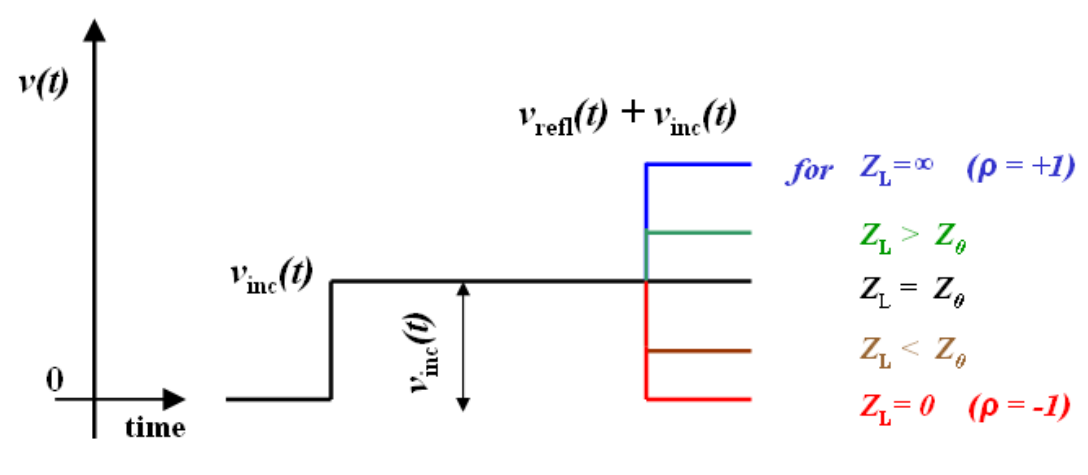
\includegraphics[width=\textwidth,keepaspectratio]{images/onereflectionsample.png}\caption{Znázornění jednoho odrazu na vedení \cite{broadbandreflectometry}.}\label{simpleresponse}\end{figure}

Postupně je možné analyzovat tuto impulzní odezvu tak, že se postupuje od okamžiku budicího signálu, až je nalezen první odraz. Z tohoto odrazu a známého budicího signálu je možné spočítat koeficient odrazu \gls{gama} a prostupu \gls{transmise} v daném místě. Dále postupuje jen množství energie definované koeficientem prostupu a energií obsažené v budicím signálu. Při znalosti této energie, koeficientu odrazu dalšího bodu, kde nastává odraz a koeficientu prostupu prvního odrazu (energie odražená od druhé diskontinuity musí opět projít první diskontinuitou). Takto se postupuje až do konce naměřených dat.

Takto jednoduchý postup ovšem zanedbává vliv vícenásobných odrazů. Přesné výsledky dává pouze pro jeden jediný (resp. první) odraz. Čím více diskontinuit na vedení se nachází, tím více se bude nalezené řešení odchylovat od reality. Pro přesnější analýzu je nezbytné, aby byly uvažovány i vícenásobné odrazy. Je možné mezi jednotlivé kroky analýzy impedančního profilu vložit další analytický krok, který zajistí odečtení vlivu vícenásobných odrazů. Tímto krokem je provedení \acrshort{FDTD} simulace s použitím již získaného částečného impedančního profilu, který je virtuálně bezodrazně zakončen. Výsledkem takovéto \acrshort{FDTD} simulace je odezva takovéhoto úseku vedení (jako průběh odraženého signálu, tak prostupujícího). Nasimulovaný odražený signál je možné odečíst od změřených dat, čímž jsou odstraněny vícenásobné odrazy v již známé části vedení. Dále se pokračuje v analýze tohoto rozdílu měřených a simulovaných dat. Dále se hledá další odraz na vedení a postup se opakuje, dokud není zpracováno celé vedení, nebo dokud energie ve vedení není všechna odražena zpět (platí pro bezeztrátová vedení). Při znalosti fázové rychlosti v daném vedení je možné přepočítat časovou osu na osu prostorovou a odhadnout tedy, kde se nachází diskontinuity.

Dále je možné z těchto odrazů zjišťovat, zda jde o odraz způsobený spojením dvou vedení o rozdílné impedanci (taková diskontinuita se vyznačuje koeficientem odrazu, který se při měření ze dvou stran jeví tak, že má z každé strany koeficient odrazu s jiným znaménkem) nebo o lokální chybu způsobenou například mechanickým poškozením vedení (například navrtaný kabel ve zdi). Taková závada by měla mít z obou stran totožné vlastnosti.

Pro zpracování obecně komplexních koeficientů odrazu (tedy například část vedení, která se chová kapacitně nebo induktivně) by bylo nezbytné vytvořit algoritmus, který by byl schopen rozeznávat v impulsní odezvě nejen čistě reálné odrazy mající v naměřených datech podobu Kroneckerova delta, ale i exponenciální průběhy odpovídající komplexním impedancím, např. na obr. \ref{complexresponse}. Takový algoritmus může být již výrazně náročnější na implementaci, neboť může vyžadovat vícerozměrnou optimalizaci k tomu, aby bylo dosaženo simulací změřené odezvy. Vyvstává také otázka, jak analyzovat, zda jde o přítomnost komplexní impedance na vedení nebo například speciálně zhotovené části vedení, která má spojitý profil impedance, který napodobuje přítomnost komplexní impedance na vedení.

\begin{figure}[htbp]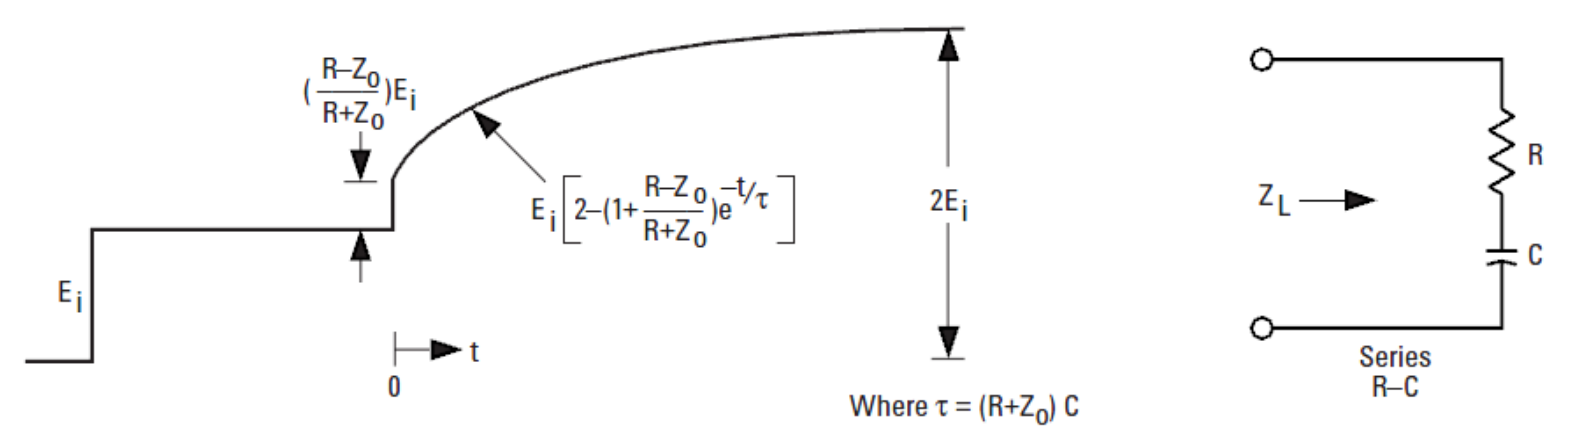
\includegraphics[width=\textwidth,keepaspectratio]{images/samplecomplexresponse.png}\caption{Příklad odezvy na komplexní impedanci na vedení \cite{broadbandreflectometry}.}\label{complexresponse}\end{figure}

Veškeré tyto úvahy se však týkají převážně bezeztrátových vedení, případně vedení, kde je snadné odhalit ztrátové prvky. Obtížné je například měření útlumu měřeného vedení, neboť samotný útlum vedení nemusí být měřitelný jako odraz. Je-li totiž vedení po celé délce homogenní, nevznikají na něm žádné odrazy, avšak vlivem ztrát dielektrika nebo konečnou vodivostí vodičů se část přenášené energie mění na teplo. Další problém je měření části vedení, která se nachází za ideálním útlumovým článkem nebo nějakým prvkem, který transformuje impedanci. Teoreticky není možné odhalit útlumový článek, pokud není možné různými způsoby zakončit vedení, aby byl odhalen vliv zakončení vedení na celkovou odezvu. I při takovém postupu však není možné určit, kde přesně se takový prvek nachází, protože na něm nevzniká žádný odraz, kterým . 

Vzhledem ke značné složitosti této analýzy je zpravidla na reflektometrech a kabelových analyzátorech přítomna pouze funkce detekce první diskontinuity, její polohy a charakteru (zkrat, rozpojení, obecně jiná impedance) \cite{CT-100Bmanual} .

Dalším tématem je měření aktivních prvků, neboť v takovém případě je možné dosáhnout koeficientu odrazu s velikostí větší než 1. V takovém případě je možné analýzou pouze zjistit přítomnost aktivního prvku a jeho odezvu, pro zjištění vlastností takového prvku (například vytvoření modelu tranzistoru) je nezbytné znát vnitřní model takového prvku, což již není úlohou reflektometru. Obecně také může být obtížné analyzovat vedení, na kterém se může nacházet nějaký nelineární prvek (takovým případem může být i například přítomnost vlhkosti ve vedení, která změní impedanci vedení, ovšem nad přibližně 3\,GHz kvůli dielektrické relaxaci přestane mít vliv \cite{relaxationspectroscopy}).

Závěrem této části práce může být tedy konstatování, že je jednoduché odhalit první diskontinuitu (nebo největší, jsou-li ostatní dostatečně malé). Obtížnější je charakterizovat ji, má-li komplexní imepdanci. Mnohem obtížnější je analýza celého vedení, v případě uvažování obecně komplexní impedance může být nemožné získat jednoznačnou analýzu takového vedení, protože může být způsobena jak komplexní impedancí na vedení, tak zvláštně vytvořenému vedení. Přítomnost nelinearit na vedení může zcela znemožnit jakoukoli analýzu nebo způsobit celkovou nesprávnost takové analýzy.

V dalších kapitolách budou rozebrány jednotlivé stavební bloky nezbytné pro konstrukci \acrshort{TDR} a možnosti jejich implementace s přihlédnutím k jednoduchosti fyzické implementace a možností následného zpracovaní naměřených dat.
\chapter{Budicí signál}

\section{Základní požadavky na vlastnosti budicího signálu}
Budicí signál musí splňovat jisté podmínky, aby jej bylo možné použít pro charakterizaci měřeného systému. Následuje formulace základních kritérií pro výběr vhodného budicího signálu.

\begin{itemize}
	\item
	\textbf{Fyzikální realizovatelnost}\\*
	Vzhledem k tomu, že navrhované zařízení musí být realizovatelné, je nezbytné, aby i budicí signál byl fyzikálně realizovatelný. Vzhledem k fyzikálním a praktickým omezením (existence materiálové disperze, nemožnost vytvoření nekonečně velkého proudu, neexistuje bezkapacitní prostředí, neexistuje bezindukční vedení, neexistuje zdroj schopný dodat nekonečné množství energie) není možné vytvořit nespojitý signál. Derivace napětí takovéhoto signálu tedy nemůže být nekonečná. Nespojité signály je tak možné pouze aproximovat spojitými signály, což omezuje například délku a strmost náběžných hran v těchto aproximovaných nespojitostech. Toto fyzikální omezení tedy omezuje frekvenční spektrum takového budicího signálu, zejména jeho šířku.
	
	\item
	\textbf{Spektrální požadavky}\\*	
	Spektrum budicího signálu by mělo být pokud možno konstantní a co nejširší. Neobsahuje-li budicí signál nějakou část spektra, není možné otestovat odezvu systému na tuto část spektra a plně tedy charakterizovat měřený systém. Důvod pro požadavek na rovné spektrum vyplývá z omezeného dynamického rozsahu reflektometru - pokud by část spektra měla příliš malou úroveň, bylo by měření v této části spektra buď více zatížené šumem, případně až neměřitelné. V případě měření některých systémů může být výhodné používat úzkopásmový signál, například při měření části systému nacházející se za pásmovou propustí. V takovém případě by mohla být odezva od části systému za pásmovou propustí maskována mnohem silnějším odrazem od propusti. Jedná se však o specifický případ, který je možné vyřešit i jinými metodami, například redukcí odrazu v nechtěném pásmu \cite{sincgausstdr}. Pro zcela obecné použití by měl být širokopásmový signál vhodnější.
	
	\item
	\textbf{Jednoduchost}\\*	
	Zvolený budicí signál by měl být jednoduchý na vytvoření. Se složitostí signálu může růst složitost zapojení, které by ho mělo generovat, jeho fyzická velikost, případně i náklady na takové zařízení.	

	\item
	\textbf{Rozlišitelnost budicího signálu od odrazů}\\*	
	Budicí signál musí být rozlišitelný od odrazů. Kupříkladu pro buzení periodickým signálem by mělo platit, že odezva měřeného systému na budicí signál musí být kratší než perioda budicího signálu. V opačném případě by se překrývala část odezvy s odezvou od další periody budicího signálu.
\end{itemize}

\section{Výběr budicího signálu a možnosti jeho syntézy}
V této části jsou uvedeny možné podoby budicích signálů a obecné možnosti jejich syntézy. Zároveň jsou zde diskutovány jejich vlastnosti a možnosti následného zpracování. U signálů jsou uvedeny i již existující implementace reflektometrů s těmito budicími signály.

\begin{itemize}
	\item
	\textbf{Diracovo delta}\\*	
	\begin{figure}[htbp]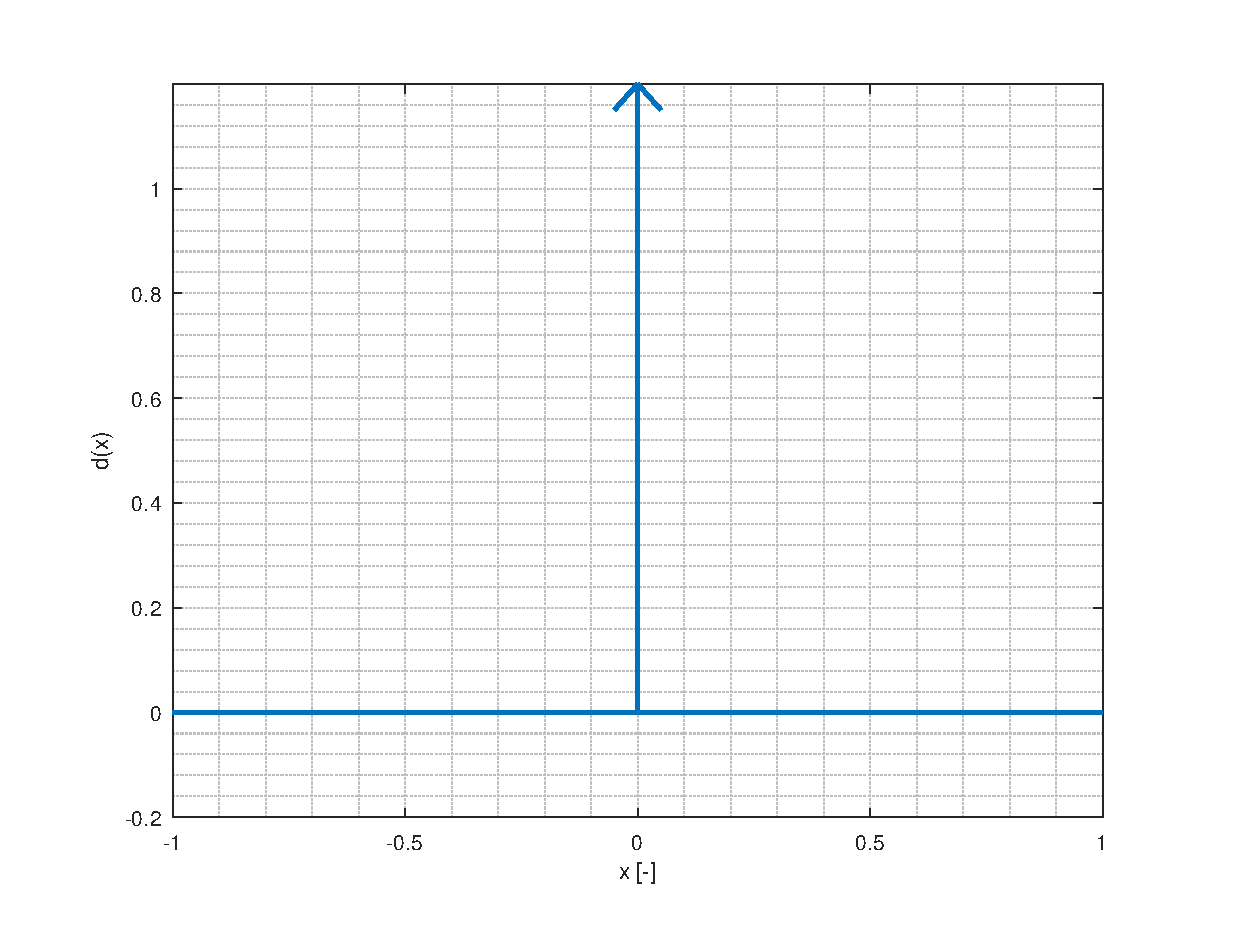
\includegraphics[width=\textwidth,keepaspectratio]{images/dirac.eps}\caption{Diracovo delta.}\label{dirac}\end{figure}		
	Diracovo delta (na obr. \ref{dirac}) je velice jednoduchý signál, který je jedním z ideálních budicích signálů, jeho spektrum je konstanta, má tedy neomezenou šířku frekvenčního pásma. Odezva na Diracovo delta odpovídá impulzní odezvě systému.  Bohužel není fyzikálně realizovatelný, jak je shrnuto v předchozí části textu, neboť je nespojitý a vyžaduje nekonečně rychlé změny napětí a proudu v obvodu. Je tedy možné pouze jej aproximovat, čímž se změní jeho spektrum. Výsledný signál bude mít spektrum odpovídající spektru Diracova delta filtrovaného dolní propustí, čímž se jeho šířka pásma omezí na konečnou velikost. Možná podoba takového signálu je Gaussův pulz na obr. \ref{gauss}.
	
	\begin{figure}[htbp]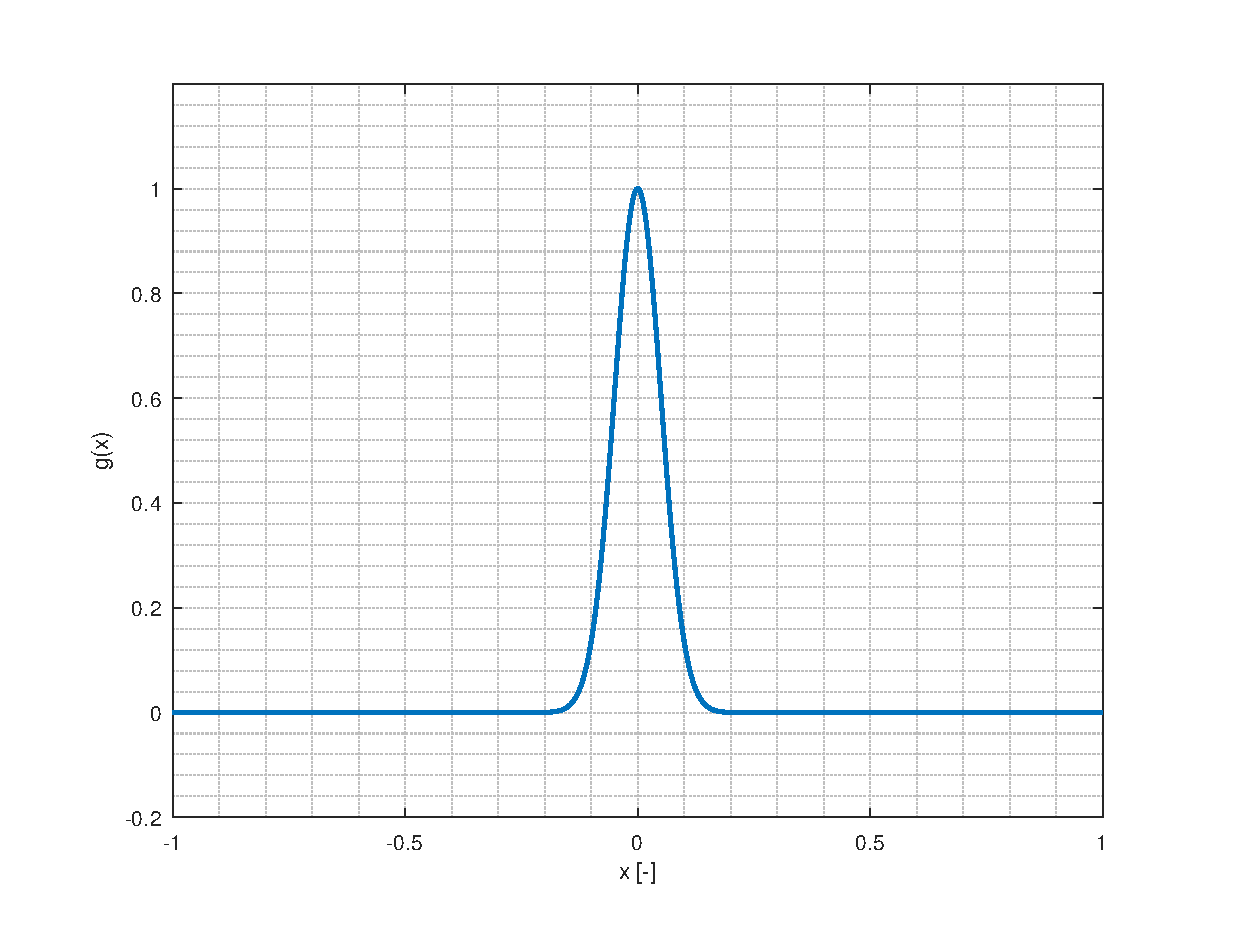
\includegraphics[width=\textwidth,keepaspectratio]{images/gauss.eps}\caption{Gaussův pulz, variance=0.05.}\label{gauss}\end{figure}			
	
	Aproximaci Diracova delta je možné vytvořit pomocí lavinových generátorů impulzů \cite{AN72LT}, \cite{AN94LT}. Pro dosažení impulzu o délce menší než stovky pikosekund je možné použít kombinaci lavinového generátoru impulzů, \acrfull{SRD} a takzvané \gls{clipline} podle obr. \ref{clipline_generator} \cite{S-4manual} \cite{S-1manual}. Takové řešení je však již prostorově náročné, protože vyžaduje zdroj lavinového napětí, transformátory a zkratovací vedení.
	
	\begin{figure}[htbp]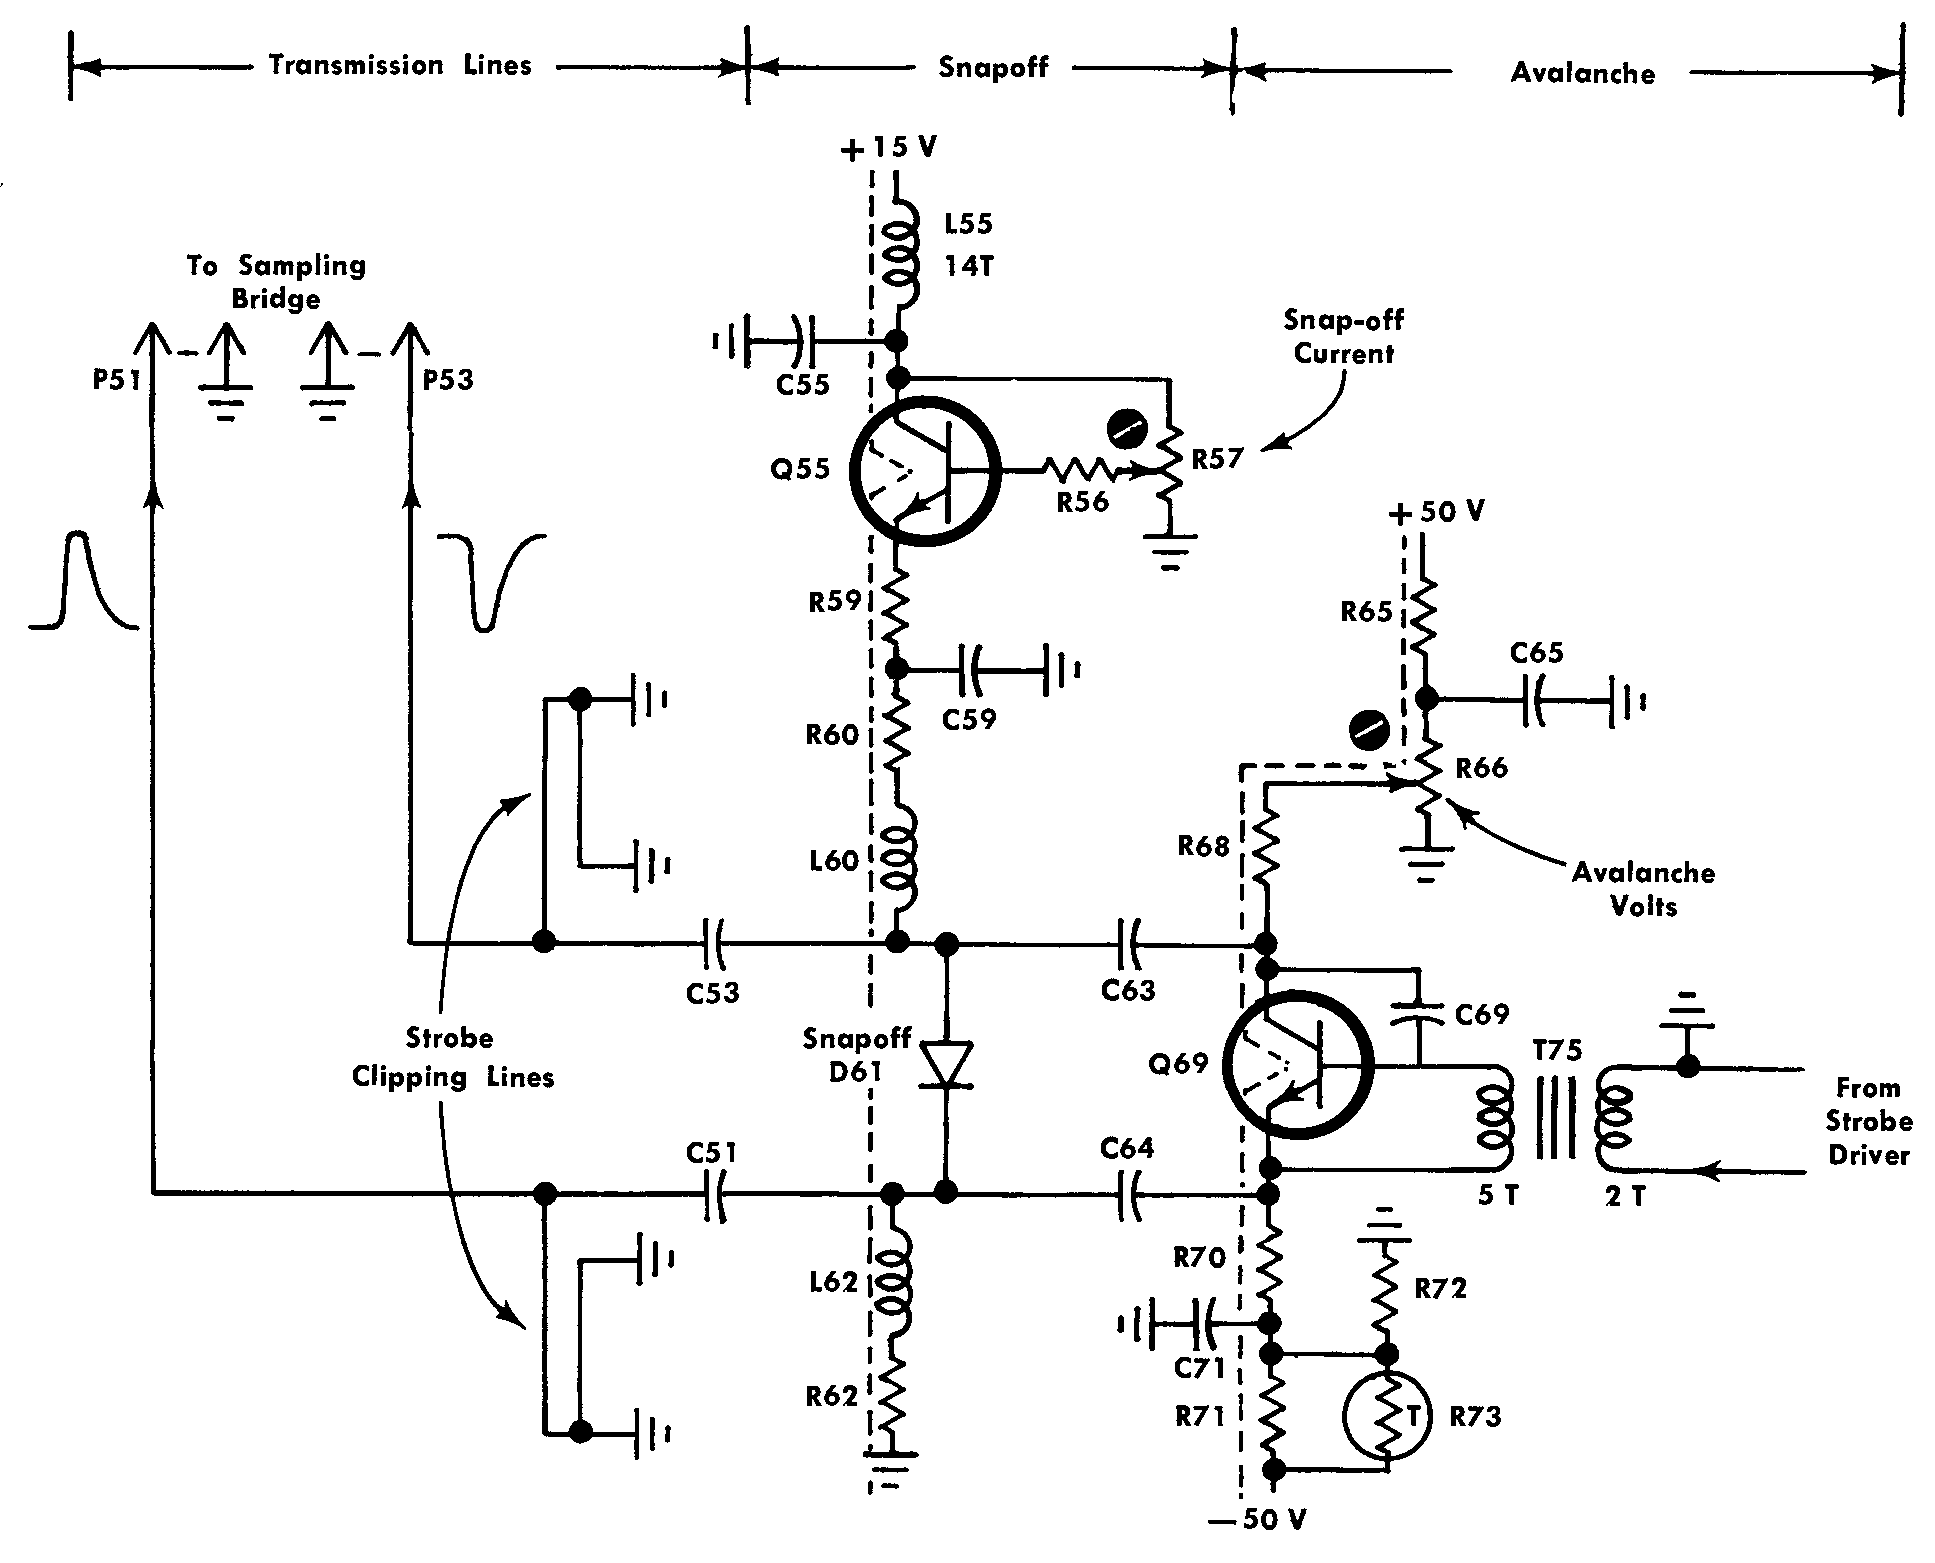
\includegraphics[width=\textwidth,keepaspectratio]{images/clipline_generator.png}\caption{Jehlový generátor s lavinovým generátorem, \acrshort{SRD} a zkratovacím vedením \cite{S-1manual}.}\label{clipline_generator}\end{figure}			
	
	\item
	\textbf{Jednotkový skok}\\*
	\begin{figure}[htbp]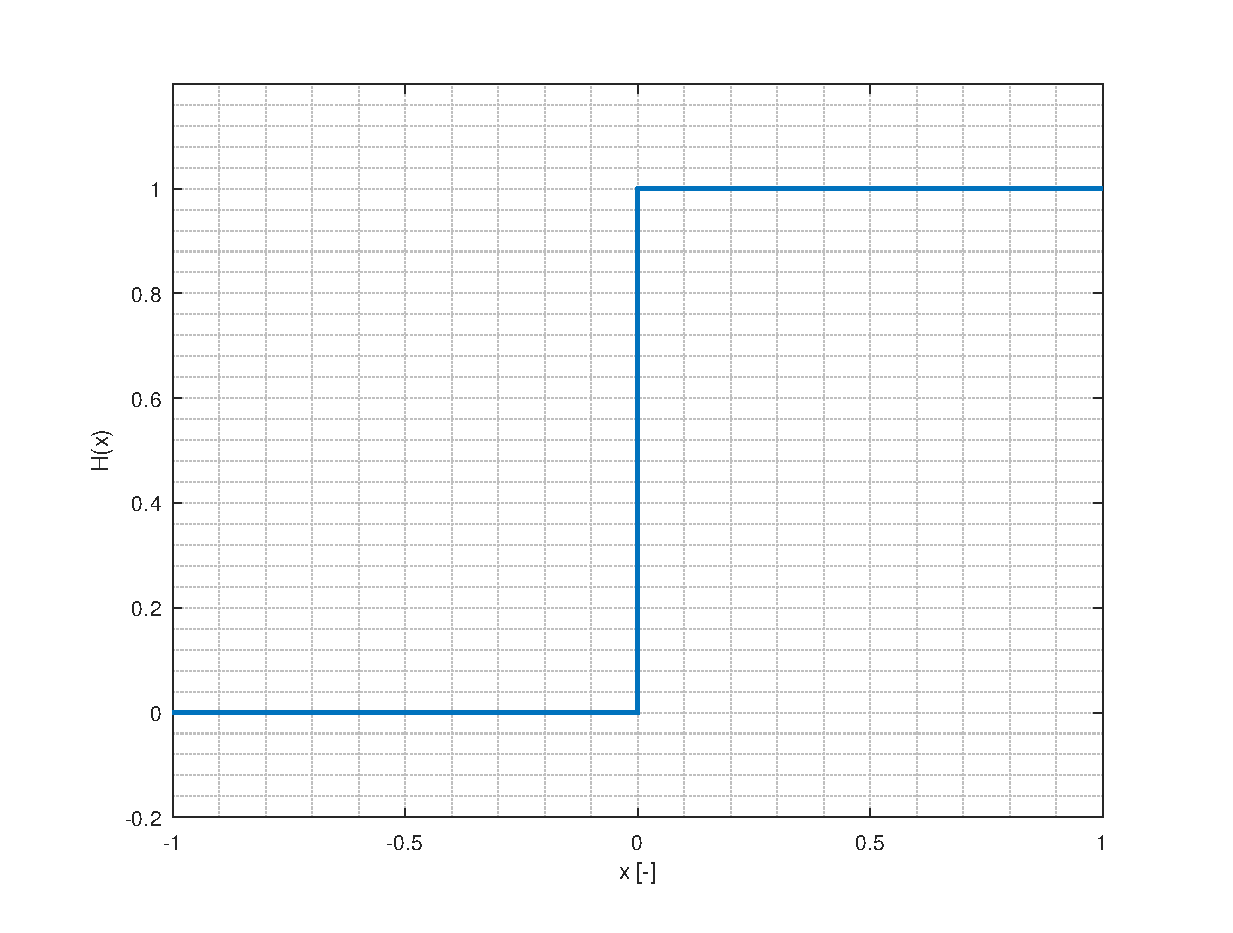
\includegraphics[width=\textwidth,keepaspectratio]{images/unitstep.eps}\caption{Jednotkový skok.}\label{unitstep}\end{figure}		
	Jednotkový skok na obr. \ref{unitstep} odpovídá časovému integrálu Diracova delta
	\begin{equation}
		H(x)=\int_{-\infty}^x \delta(t) dt.
	\end{equation} Opět se jedná o nespojitý signál, který nejde realizovat, jen aproximovat. Reálná aproximace jednotkového skoku je například chybová funkce $\erf(x)$ na obr. \ref{errorfunction}.
	
	\begin{figure}[htbp]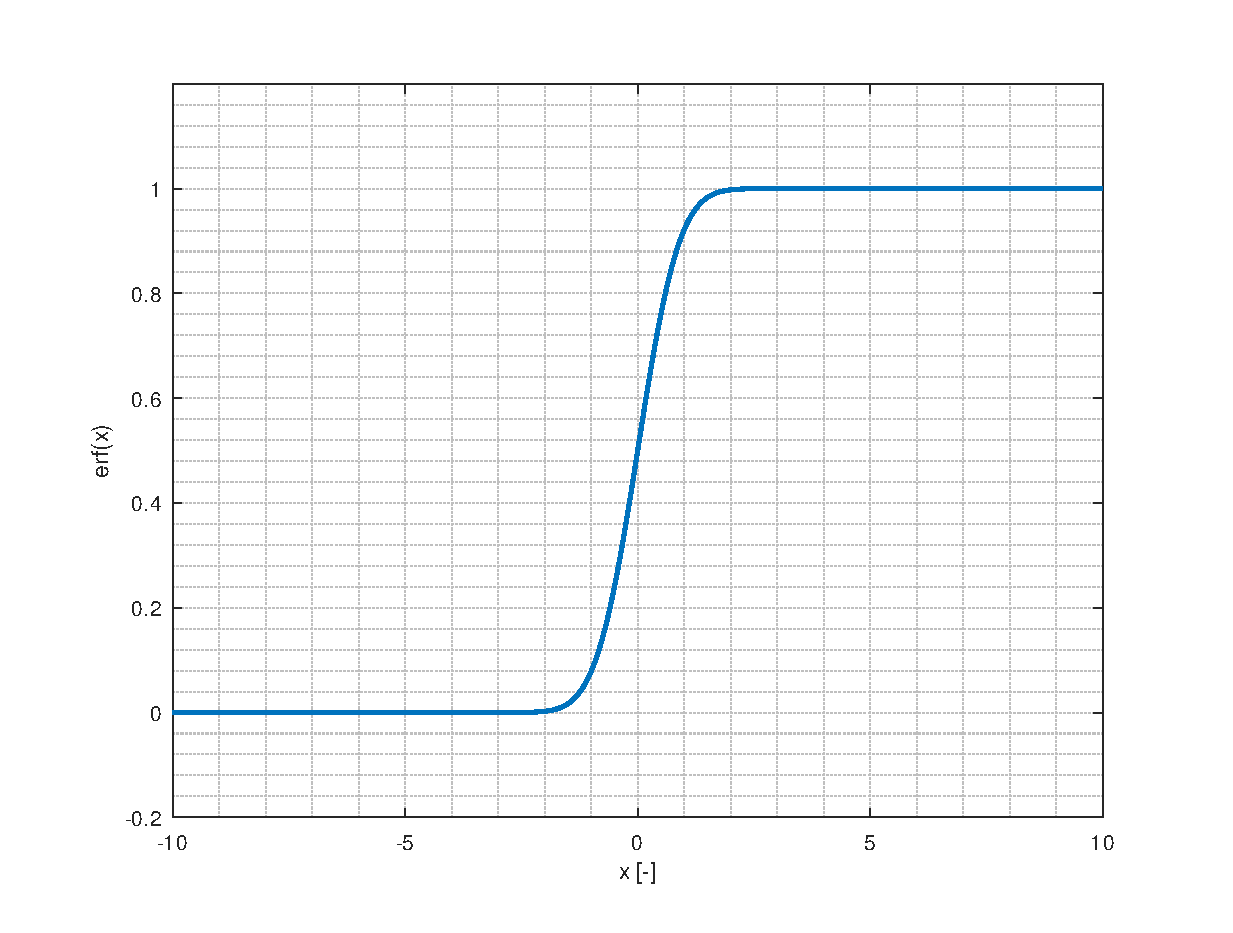
\includegraphics[width=\textwidth,keepaspectratio]{images/erf.eps}\caption{Chybová funkce.}\label{errorfunction}\end{figure}		
		
	Tento budicí signál je možné jednoduše generovat pomocí rychlých logických obvodů. Moderní logické obvody používané pro vysokorychlostní spoje (\acrshort{SATA}, \acrshort{SAS}, \acrshort{USB}\,3, \acrshort{PCI-E}) v řádu jednotek \si{\giga\bit\per\second} již mají náběžné hrany o délce kratší než 100 ps \cite{SY54017datasheet}, \cite{SN75LVCP600Sdatasheet}, \cite{SN65LVPE501datasheet}, \cite{TUSB1002Adatasheet}. Vzhledem k tomu, že pro převod skokové odezvy na impulsní je možné použít jednoduchý vztah
	\begin{equation}
	h(t)=\dv{a(t)}{t},
	\end{equation} a že je syntéza jednotkového skoku možná přímo pomocí logického obvodu, je výhodnější použít jednotkový skok než Diracovo delta. Pravděpodobně z těchto důvodů se u běžných reflektometrů používá právě jednotkový skok jako budicí signál.
	
	\item
	\textbf{Funkce $\boldsymbol{\sinc(x)}$}\\*	
	\begin{figure}[htbp]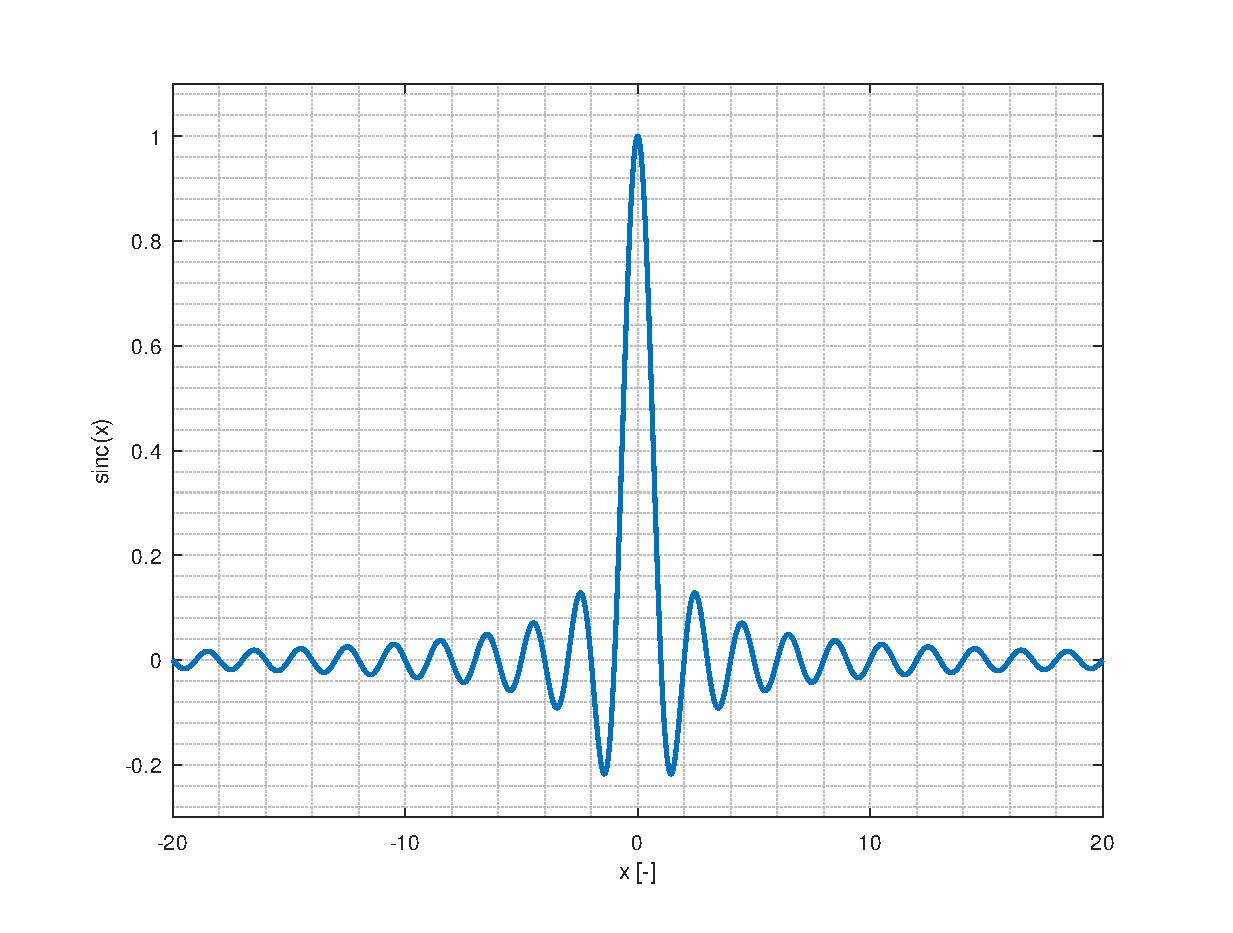
\includegraphics[width=\textwidth,keepaspectratio]{images/sinc.eps}\caption{Funkce $\sinc(x)$.}\label{sinc}\end{figure}		
	
	Další možný budicí signál je funkce $\sinc(x)$ na obr. \ref{sinc}. Tato je již idealizovaně fyzikálně proveditelná (musela by být nekonečně dlouhá), spektrum funkce je konstantní až do mezní frekvence, dále je nulové. Vzhledem k ostrému omezení spektra bohužel není možné změřenou odezvu převést na impulsní odezvu, což komplikuje další zpracování. Autokorelace této funkce je opět $\sinc(x)$, není tedy možné takto jednoduše takovouto odezvu analyzovat.
	
	Pro vytvoření průběhu funkce $\sinc(x)$ je možné modulovat harmonický signál obálkou \cite{sincgausstdr}, ovšem taková obálka by musela být přesně synchronizována s nosným harmonickým signálem, aby nedocházelo ke zkreslení spektra. Jedna z možností, jak přesně simulovat tuto funkci je přímá digitální syntéza, pro tu by ovšem bylo nezbytné použít obvod \acrshort{DDS} s hodinovou frekvencí nejméně dvakrát větší než požadované pásmo, tedy vyšší jednotky GHz. Tento signál nenabízí tedy ani snadnou implementaci, ani vhodné vlastnosti pro použití jako buzení.
	
	\item
	\textbf{Bílý šum}\\*	
	\begin{figure}[htbp]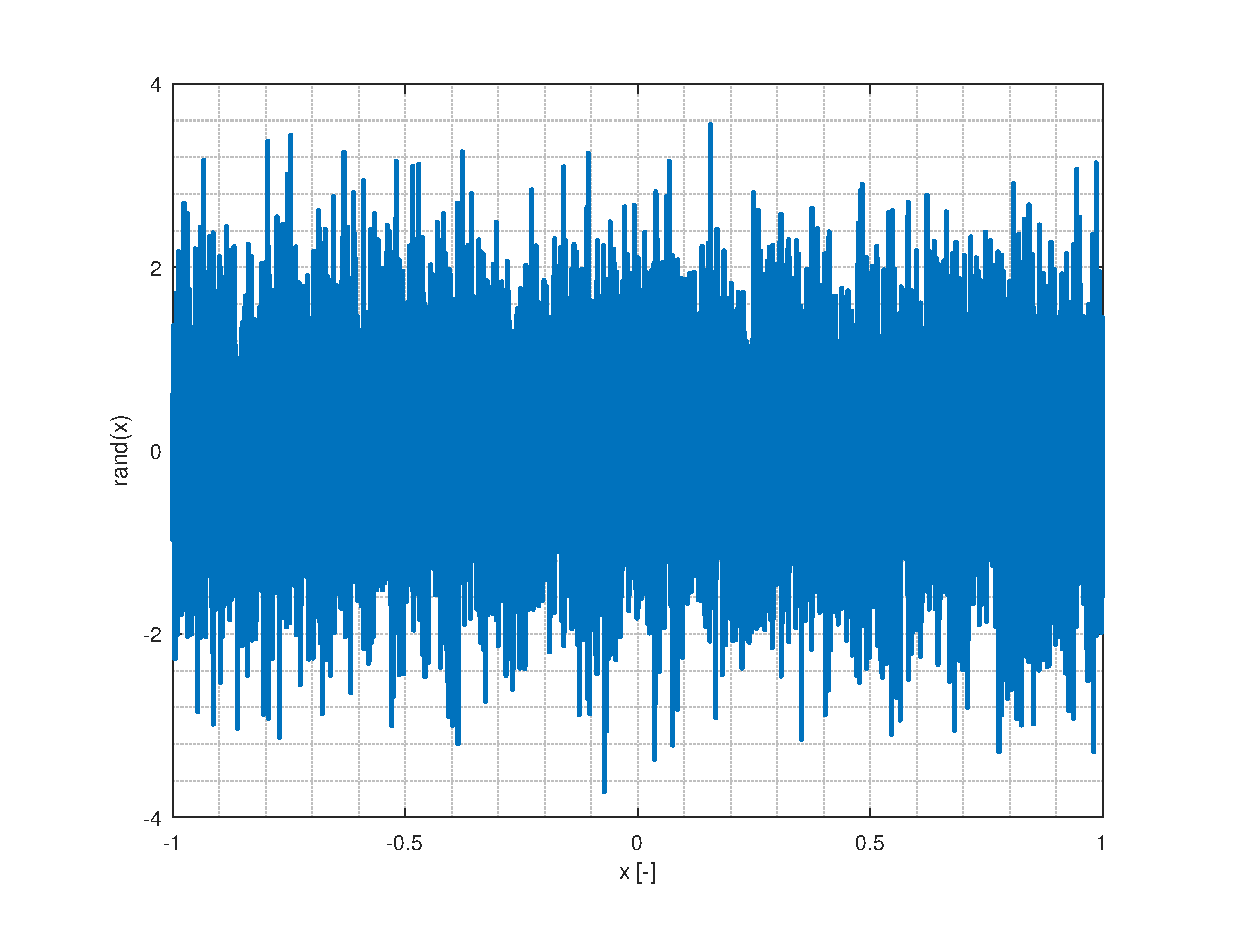
\includegraphics[width=\textwidth,keepaspectratio]{images/whitenoise.eps}\caption{Diskrétní bílý šum.}\label{whitenoise}\end{figure}			
	Při použití bílého šumu (obr. \ref{whitenoise}) je možné získat impulsní odezvu pomocí autokorelace odezvy soustavy. Taková operace zároveň může potlačit nežádaný šum. Pro použití bílého šumu by ale bylo nezbytné, aby budicí šum byl rozlišitelný od šumu nežádaného. Toho lze dosáhnout například zapínáním a vypínáním budicího šumu.
	
	\begin{figure}[htbp]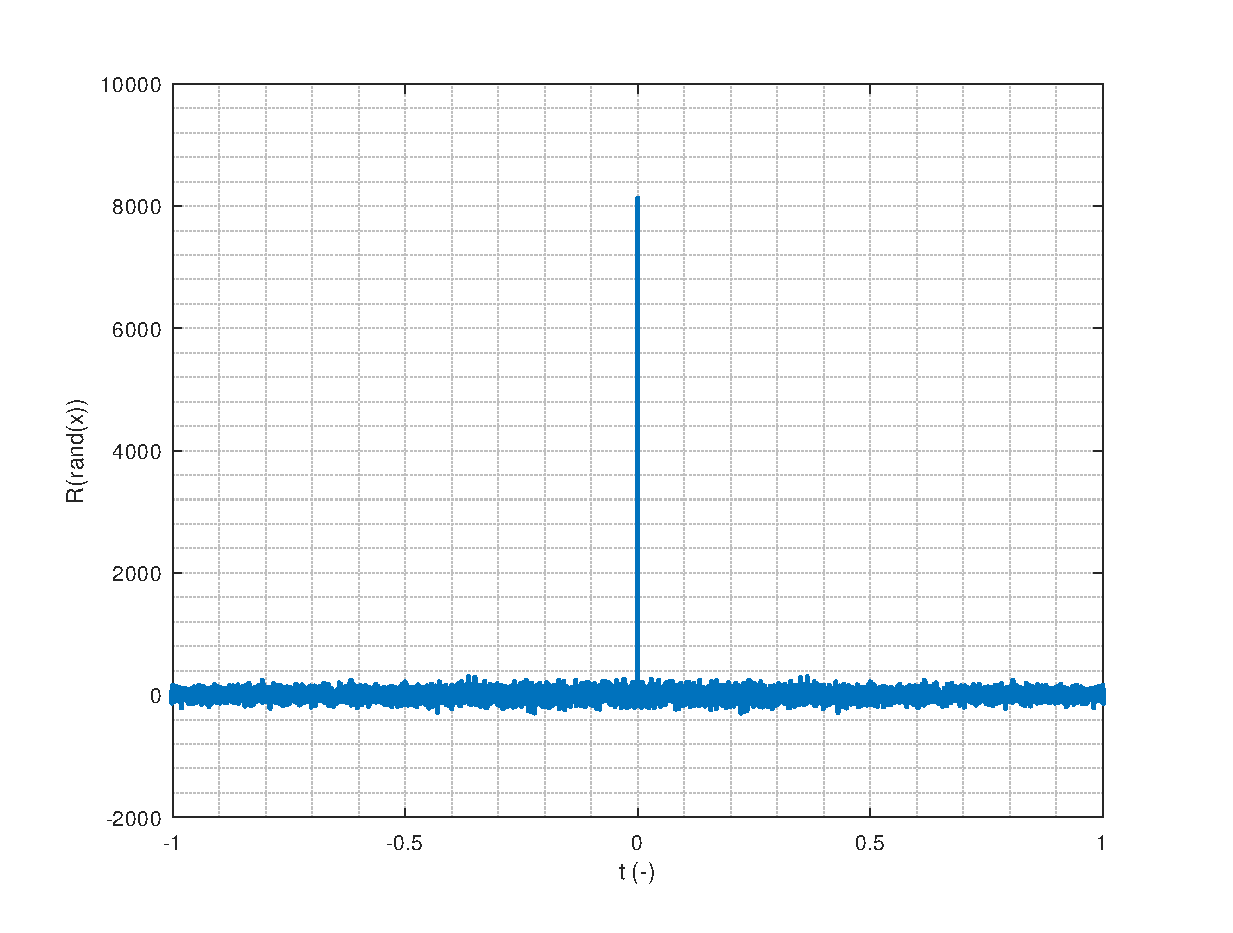
\includegraphics[width=\textwidth,keepaspectratio]{images/whitenoisecorr.eps}\caption{Autokorelace diskrétního bílého šumu z \ref{whitenoise}.}\label{whitenoisecorr}\end{figure}		
	
	Širokopásmový šum je také možné jednoduše vytvořit, například pomocí šumových diod. Modulaci tohoto šumu je možné provádět například pomocí polovodičových mikrovlnných přepínačů. Takový budicí signál je tedy možné jednoduše vytvořit i zpracovávat. Podstatná nevýhoda bílého šumu spočívá v náhodnosti, a z toho vyplývající neperiodicity, kvůli které není možné odezvu systému na takový signál měřit v ekvivalentním čase, jen v reálném čase. Je možné ovšem rovnou měřit autokorelaci, tedy násobením odezvy systému se zpožděnou kopií, kterou je možné vzorkovat pomalu. Autokorelace diskrétního bílého šumu se nachází na obr. \ref{whitenoisecorr}. Bohužel takový přístup vyžaduje použití zpožďovacího vedení s proměnnou délkou, které musí být buď vytvořeno jako mechanický pohyblivý díl nebo jako vedení s velkým množstvím odboček, pak ale je časový krok měření omezen polohou odboček a celková délka měření je omezena délkou vedení \cite{noisedomainreflectometry}. Tuto metodu měření je možné použít pro měření na vedení, na kterém se nachází aktivní zařízení, protože nežádané signály je možné do velké míry odfiltrovat autokorelací. Tato metoda může být tedy výhodná pro měření na předem známých systémech (pevná nehybná vedení), například ve strojích, továrnách, dopravních prostředcích, pro obecné použití se však nezdá být praktická. 
	
	\item
	\textbf{Deterministický šum}\\*
	Za deterministický šum je možné považovat například vedení, které slouží k digitální komunikaci, přičemž obsah posílaných zpráv je známý nebo se tyto zprávy opakují. Pro měření touto metodou je však nezbytná znalost konkrétního měřeného systému \cite{noisedomainreflectometry}, nejde tedy o všeobecně použitelou metodu. 
\end{itemize}

\section{Zvolený budicí signál a obvodové řešení}
Pro jednoduchost syntézy a dobré vlastnosti byl vybrán jednotkový skok. Kvůli rychlostním požadavkům není možné použít klasické logické obvody z řad \acrshort{TTL}, \acrshort{CMOS}, \acrshort{LVCMOS}, \acrshort{HCMOS}, \acrshort{ECL} apod. kvůli velké délce náběžné hrany \cite{subnanosecondgeneratorcomparison}. U těchto technologií je náběžná hrana zpravidla delší než \SI{1}{\nano\second}. Vzhledem k vývoji dnešní techniky, zejména v oblasti vysokorychlostních digitálních přenosů, však již existují velice rychlé logické obvody schopné dosahovat náběžných hran o délce kratší než \SI{100}{\pico\second}. Ve všech dnešních počítačích se již nacházejí technologie jako \acrshort{USB}\,3, \acrshort{HDMI} nebo Display Port, \acrshort{PCI-E}, \acrshort{SATA} nebo \acrshort{SAS} (v serverech), které právě takové obvody vyžadují, díky čemuž jsou dnes již tyto obvody velmi levné. Tyto technologie jsou zpravidla pevně spojeny s metodou signalizace. Používané metody jsou vždy symetrické kvůli šumové odolnosti, používají signalizaci o rozkmitu řádově stovek milivoltů kvůli rychlosti a vyzařování do okolí. 

Běžně používané signalizační technologie:
\begin{itemize}
	\item
	\textbf{\acrshort{LVPECL}}\\*	
		Nízkonapěťová varianta dřívějšího \acrshort{ECL}, která je navíc referencovaná vůči kladnému napájecímu pólu. Vnitřní zapojení je uvedeno na schématu \ref{lvpecl_output}. Jsou navrženy pro připojení k impedanci \SI{50}{\ohm}, bohužel výstupní budiče jsou zapojeny jako emitorové sledovače \cite{lvpecl_vml_cml_lvds_interfacing}, jsou tedy silně nelineární, nemají definovanou impedanci a nejsou tedy vhodné jako budicí obvod do reflektometru, neboť v reflektometru se vyžaduje dobré přizpůsobení měřicího portu, tedy jeho impedance musí být přesně definovaná a konstantní, navíc není žádoucí, aby se měřicí port choval nelineárně.
	
		\begin{figure}[htbp]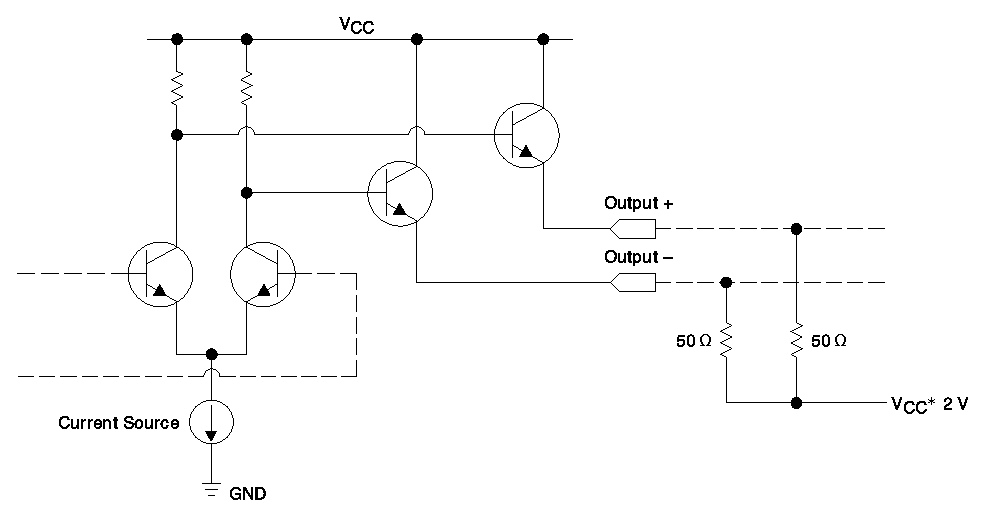
\includegraphics[width=\textwidth,,height=10cm,keepaspectratio]{images/lvpecl_output.eps}\caption{Typické zapojení LVPECL výstupu, převzato \cite{lvpecl_vml_cml_lvds_interfacing}.}\label{lvpecl_output}\end{figure}		
		
	\item
	\textbf{\acrshort{LVDS}}\\*
		Tato signalizace se běžně používá pro přenos obrazu po \acrshort{HDMI} nebo Display Port. Se zmenšeným rozkmitem (\SI{250}{\milli\volt}) se používá i pro \acrshort{SATA} a \acrshort{SAS}.  Vnitřní zapojení je uvedeno na schématu \ref{lvds_output}. Výstupní budiče jsou zapojeny jako \acrshort{CMOS} push-pull budiče \cite{lvpecl_vml_cml_lvds_interfacing} zapojené do drainů tranzistorů, velice podobné jsou i budiče technologie \acrshort{VML} \cite{lvpecl_vml_cml_lvds_interfacing} a \acrshort{HCSL}, očekává se diferenciální zakončení přibližně \SI{100}{\ohm}, případně $2\times\SI{50}{\ohm}$ s pevným středem. Tyto budiče by měly být méně nelineární než \acrshort{LVPECL}, opět však zpravidla není výstupní impedance garantována.
		
		\begin{figure}[htbp]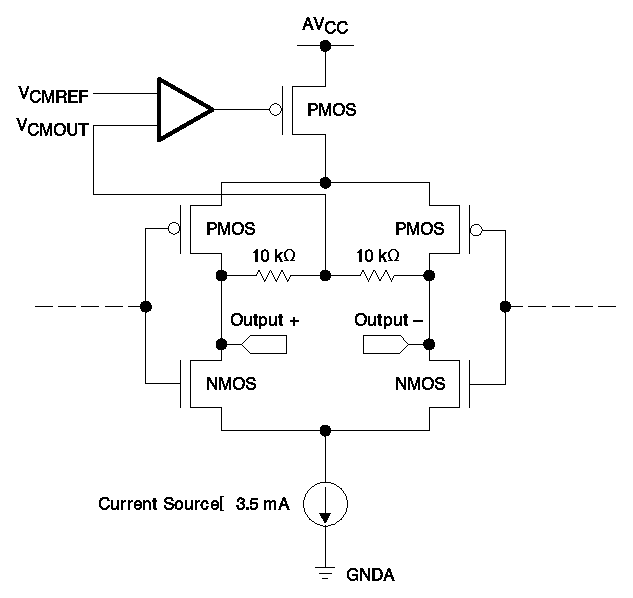
\includegraphics[width=\textwidth,height=8cm,keepaspectratio]{images/lvds_output.eps}\caption{Typické zapojení \acrshort{LVDS} výstupu, převzato z  \cite{lvpecl_vml_cml_lvds_interfacing}.}\label{lvds_output}\end{figure}	

	\item
	\textbf{\acrshort{CML}}\\*
		\acrshort{CML} je signalizační standard používaný zejména pro přenos hodinových signálů. Vnitřní zapojení je uvedeno na schématu \ref{cml_output}. Výstupní budiče jsou zapojeny do kolektoru resp. drainu tranzistoru \cite{lvpecl_vml_cml_lvds_interfacing}, jsou terminovány na \SI{50}{\ohm}, tato hodnota a její tolerance bývá garantována \cite{SY54017datasheet}. Vzhledem k zapojení do kolektoru a interní terminaci je takovýto budič velice dobře přizpůsobený k \SI{50}{\ohm} vedení. 
	
		\begin{figure}[htbp]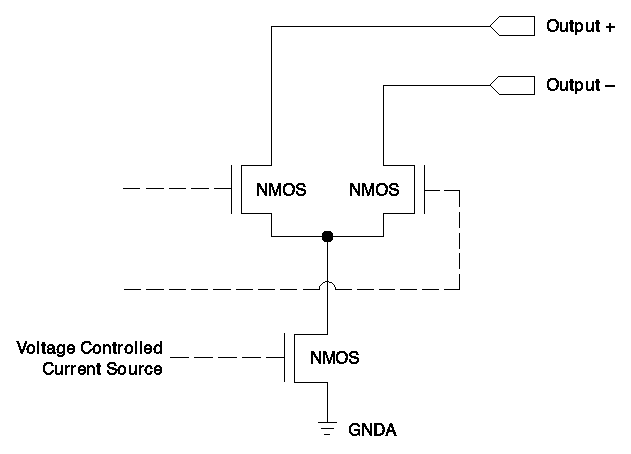
\includegraphics[width=\textwidth,height=8cm,keepaspectratio]{images/cml_output.eps}\caption{Typické zapojení \acrshort{CML} výstupu, převzato z \cite{lvpecl_vml_cml_lvds_interfacing}.}\label{cml_output}\end{figure}		
		
	\item
	\textbf{\acrshort{USB}}\\*
		Další signalizační standard používá například USB, ovšem standard \acrshort{USB}\,3.0 \cite{usb30standard} nespecifikuje přímo technologii, jak této signalizace dosáhnout. Vzhledem k této nejasnosti byly USB redrivery vyřazeny z výběru.
\end{itemize}

Kvůli dobrému přizpůsobení, linearitě a vysoké rychlosti byla zvolena technologie \acrshort{CML}. Další výhodou je, že některým \acrshort{CML} logickým členům je možné měnit napájecí napětí výstupních budičů \cite{SY54020datasheet}. Nejrychlejší dostupné \acrshort{CML} budiče mají typickou délku náběžné hrany \SI{60}{\pico\second} (garantovaný rozsah \mbox{\SIrange{30}{95}{\ps}}, uvádí se pro \mbox{\SIrange{20}{80}{\%}} konečného napětí) \cite{SY54020datasheet}, \cite{SY54017datasheet}. Jsou přímo určeny pro digitální přenosy o rychlostech v řádu \si{\gigabitpersecond}. Tyto budiče tedy splňují požadavek na šířku pásma budicího signálu.
Další důvod pro použití technologie \acrshort{CML} je ten, že \acrshort{SATA}/\acrshort{SAS}/\acrshort{USB} redrivery obvykle obsahují i logiku, která detekuje, zda je přítomen validní signál odpovídající danému přenosovému médiu a v případě, že jej nedetekují, přejdou do úsporného režimu. Přesná metoda, jak je toto spojení detekováno, není zpravidla popsána, hrozilo by tedy, že by se mohl redriver chovat nedefinovaně. Další problém těchto redriverů je to, že jsou určeny pro kompenzaci vlivu frekvenční charakteristiky a ztrát na FR-4 substrátu, takže výsledný signál není prostý obdélníkový průběh, ale složitější stupňovitý průběh jako na obr. \ref{redriver} \cite{SN75LVCP601datasheet}.

		\begin{figure}[H]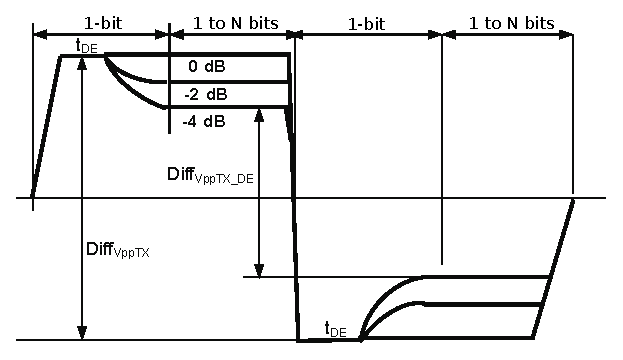
\includegraphics[width=\textwidth,height=6cm,keepaspectratio]{images/redriver.eps}\caption{Výstupní průběh \acrshort{SATA} redriveru \cite{SN75LVCP601datasheet}.}\label{redriver}\end{figure}		

\chapter{Vzorkování odraženého signálu}
Má-li být doržen Nyquistův vzorkovací teorém, je nezbytné vzorkovat budicí a odražený signál na nejméně dvakrát větší frekvenci, než se nachází nejvyšší frekvenční složka měřených signálů. Vybraný zdroj budicího signálu má šířku frekvenčního pásma až \SI{9}{\giga\hertz}, je tedy nezbytné, aby vzorkovač byl schopen vzorkovat alespoň na \SI{18}{\gigasample}. Tento vztah platí při zanedbání frekvenční charakteristiky vzorkovače, který se může chovat jako dolní propust, a tedy minimální vzorkovací frekvence může být nižší. Takovýmto vzorkovacím frekvencím se však blíží jen \quotedblbase folding\textquotedblleft{} ADC a Flash \acrshort{ADC}, které však při takovýchto rychlostech jsou nanejvýš osmibitové, tedy nabízejí dynamický rozsah nanejvýš \SI{48}{\deci\bel}. Nejrychlejší převodníky zatím (v roce 2019) nedosahují vzorkovacích frekvencí ani \SI{10}{\giga\hertz} při dostatčném dynamickém rozsahu. Pro rychlejší vzorkování se používá tzv. \gls{ADCinterleave}, tedy prokládání většího počtu převodníků. Pro přenos a zpracování dat z takto rychlých převodníků jsou potřeba i velmi rychlá FPGA, případně ještě signálové procesory. Tato metoda je ve výsledku v současné době velmi nákladná, navíc má malý dynamický rozsah.

Od doby prvních digitálních osciloskopů se používá technika známá jako vzorkování v \quotedblbase ekvivalentním čase\textquotedblleft . Tato metoda spočívá ve vzorkování periodického signálu přes větší množství jeho period, přičemž postupně se doplňují změřené body, dokud nejsou nalezeny všechny body měřeného průběhu. Hlavní nevýhoda tohoto postupu je nemožnost vzorkování jednorázových signálů (např. šum). Zásadní výhoda tohoto postupu je ovšem možnost částečně potlačit rušení z okolí, jsou-li asynchronní vůči vzorkování. Případně je možné i zvětšit dynamický rozsah, je-li použit rychlý vzorkovač pro navzorkování signálu pro pomalejší vícebitový \acrshort{ADC}. Existují dva základní přístupy, jak provádět toto vzorkování:
\begin{itemize}
	\item
		\textbf{Náhodné vzorkování}\\*		
		Vzorky jsou odebírány neustále, je zaznamenáván časový rozdíl mezi spouštěcí událostí (zde začátek budicího signálu) a nejbližší následující periodou vzorkovacího hodinového signálu. Postupně se tak náhodně doplňují naměřené body, až vznikne dostatečně přesný obraz měřeného signálu. Tato metoda je vhodná například pro osciloskopy, protože zpravidla není možné synchronizovat přesně vzorkovací hodinový signál se spouštěcí událostí.
		
	\item
		\textbf{Postupné vzorkování}\\*
		Vzorky jsou odebírány při každé periodě měřeného průběhu tak, že jednotlivé odebrané vzorky jsou časově seřazeny. Toho se dá dosáhnout fázovým posouváním vzorkovacího hodinového signálu oproti spouštěcí události, což je možné udělat pomocí digitálních zpožďovacích linek nebo tak, že vzorkovací hodinový signál a budicí signál budou mít nepatrně jinou frekvenci \cite{vernierreflectometer}. První řešení může být jednodušší na implementaci, ale zpožďovací linka omezuje krok měření a maximální počet odebraných vzorků \cite{fpgadelaylinereflectometer}, \cite{simpledelaylinereflectometer}. Druhé řešení se dá vytvořit pomocí \acrshort{DDS} \cite{ddsfpgareflectometer} nebo fázového závěsu, který podporuje násobení nebo dělení frekvencí neceločíselným násobkem. Do nedávné doby nebylo řešení pomocí fázových závěsů praktické, protože vyžadovalo fázový závěs pro vytvoření vysokofrekvenční reference a další dva fázové závěsy pro vytvoření dvou rozdílných frekvencí. V posledních letech se však objevily fázové závěsy, které všechny tyto funkce (včetně \acrshort{VCO}) integrují do jediného integrovaného obvodu a prakticky vyžadují pouze kmitočtovou referenci v podobě krystalu nebo krystalového oscilátoru \cite{ADF4350datasheet}, \cite{Si5351datasheet}.
\end{itemize}

\begin{figure}[htbp]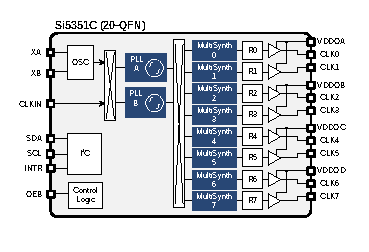
\includegraphics[width=\textwidth,keepaspectratio]{images/si5351_internal_architecture_overview.eps}\caption{Blokové zapojení \acrshort{PLL} Si5351 \cite{Si5351datasheet}.}\label{5351blockdiagram}\end{figure}

Vzhledem k existenci dostupných fázových závěsů umožňujících velkou integraci a miniaturizaci zapojení bylo zvoleno postupné vzorkování pomocí fázového závěsu. Vybraný fázový závěs Si5351 obsahuje v jednom pouzdře dva neceločíselné fázové závěsy \cite{Si5351datasheet}, dva vysokofrekvenční \acrshort{VCO} a osm výstupních neceločíselných děliček. Díky tomuto vývoji v integraci je možné celý hodinový generátor zmenšit do podoby jednoho integrovaného obvodu, jedinou potřebnou externí součástkou je krystal nebo krystalový oscilátor. Neceločíselná část násobiče frekvence umožňuje krok po $2^{{-20}}$ referenční frekvence, je tedy možné měnit podíl frekvencí hodinových signálů s krokem menším než \SI{1}{\ppm}. Při rozdílu frekvencí \SI{1}{\ppm} je počet vzorkovaných bodů celkem 1\,000\,000, což je počet bodů, který je prakticky nedosažitelný se zpožďovacími linkami.

\section{Obvodové řešení vzorkovače}
Pro měření je potřeba vzorkovač s velkou šířkou pásma, nezbytný je i malý \gls{aperturetime}. Historicky se pro tyto účely používaly diodové vzorkovače \cite{S-1manual}, \cite{S-4manual}, příklad takového zapojení na obr. \ref{oscilloscopefrontend}. V dnešní době existují již dostatečně rychlé track-and-hold zesilovače \cite{highspeed_trackhold}, tedy zesilovače, které je možné řízeně zastavit, přičemž na jejich výstupu zůstane napětí, které se tam nacházelo v okamžiku vypnutí zesilovače. Mezní kmitočet běžně prodávaných typů se pohybuje v současné době okolo \SI{8}{\giga\hertz}. Bohužel jsou oproti diodovým vzorkovačům velice nákladné.

\begin{figure}[htbp]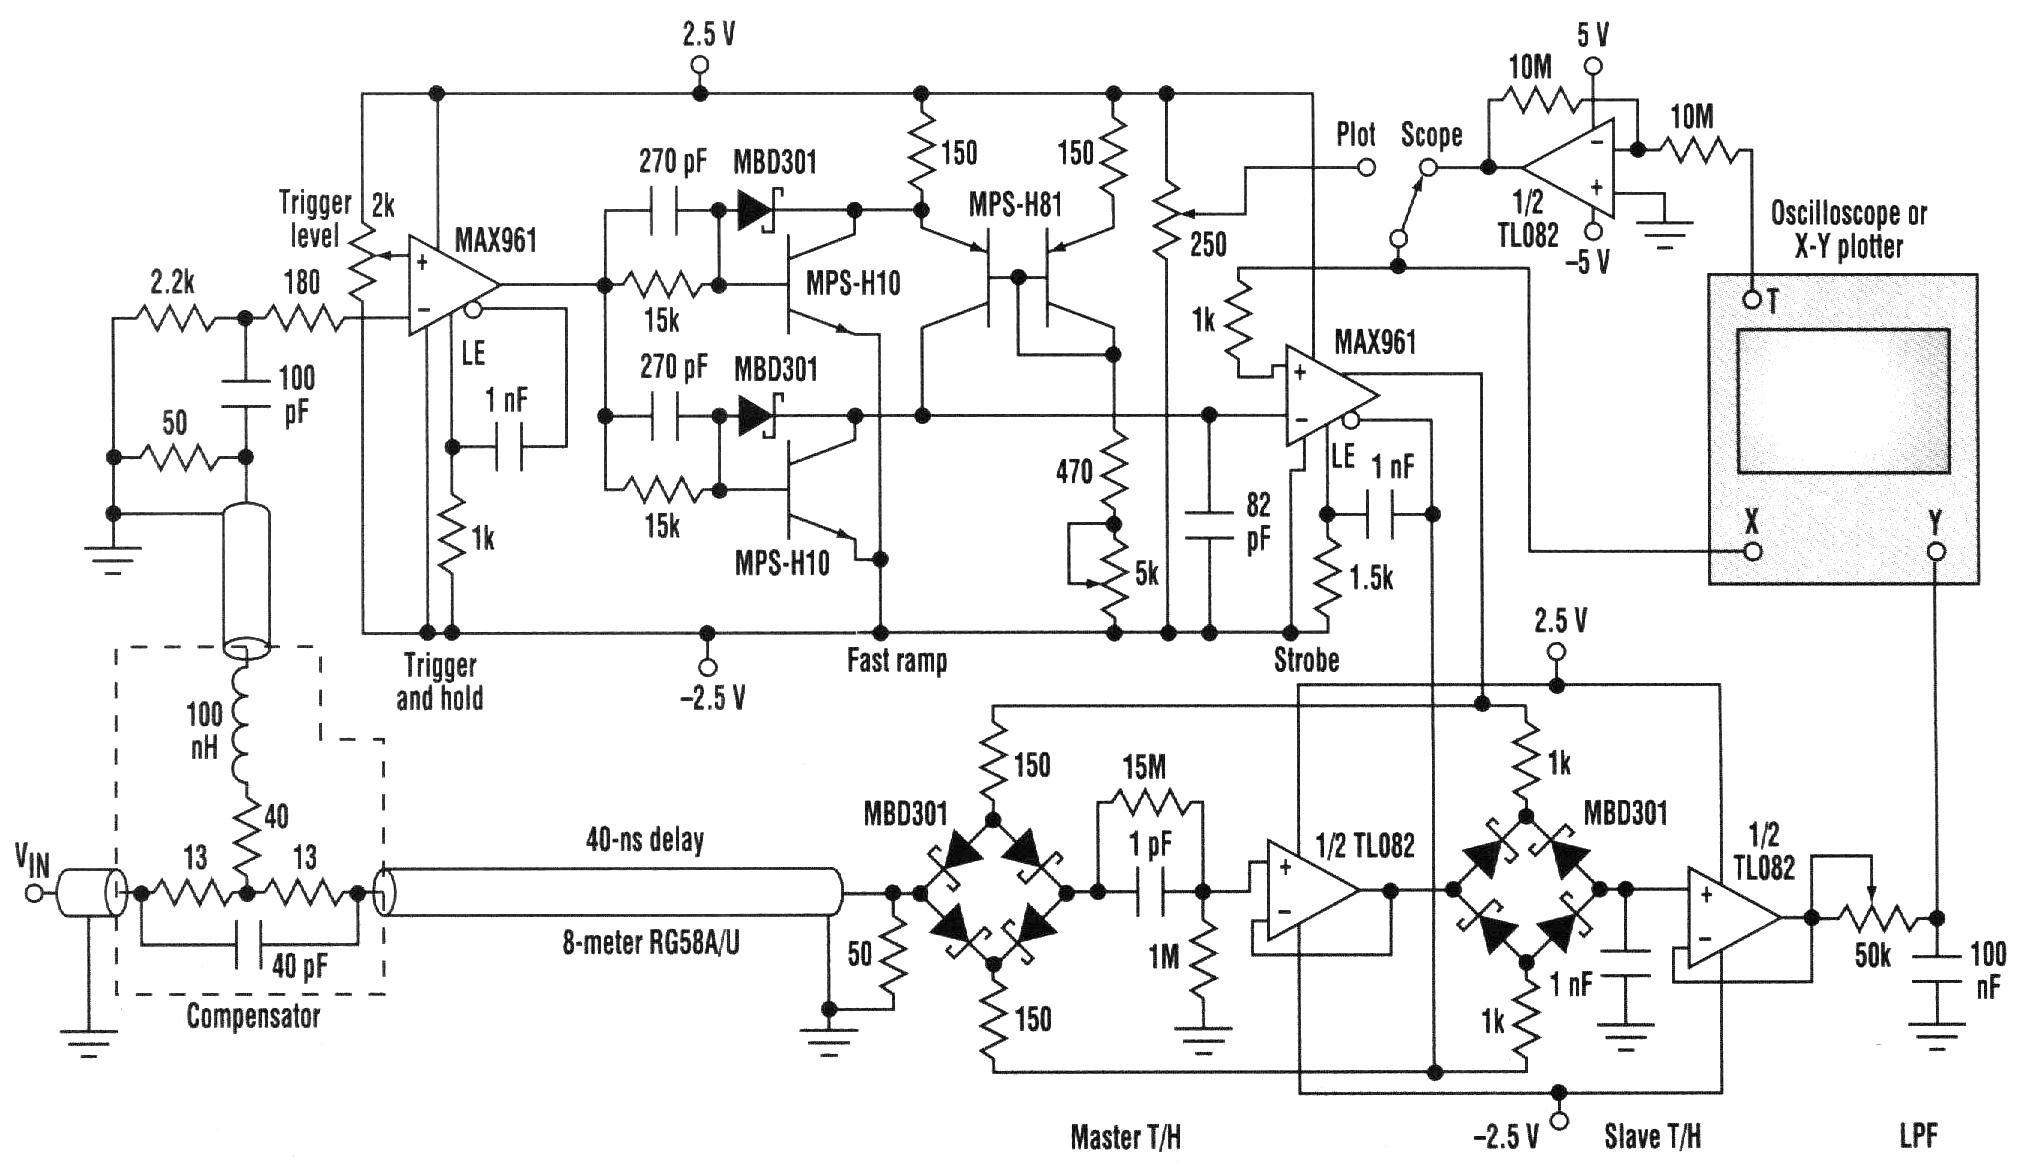
\includegraphics[width=\textwidth,keepaspectratio]{images/oscilloscopefrontend.png}\caption{Praktické zapojení vzorkovacího můstku do \SI{1}{\giga\hertz}, převzato z \cite{oscilloscopefrontend}.}\label{oscilloscopefrontend}\end{figure}		

Diodové vzorkovače se používaly již v prvních digitálních osciloskopech a reflektometrech, protože jejich šířka použitelného frekvenčního pásma je omezena téměř výhradně sériovým dynamickým odporem diodového vzorkovače, velikostí vzorkovacího kondenzátoru a aperturovým časem. Aperturový čas je doba, po kterou trvá rozepnout vzorkovač, závisí zejména na kapacitě diody (bariérové i difuzní) a zapojení budiče, který diody rozepíná. Pro toto použití jsou zejména vhodné Schottkyho diody kvůli malé paralelní kapacitě a možnosti velice rychle diody rozepnout. Speciálně pro použití ve vzorkovačích se vyrábí přesné vyvážené diodové čtveřice \cite{HSMS282xdatasheet}, které umožňují silně potlačit průnik vzorkovacího buzení do vzorkovaného signálu, což umožňuje použití velmi malých vzorkovacích kondenzátorů, a tedy velkou šířku užitečného frekvenčního pásma takového vzorkovače.
	
\chapter{Separace budicího a odraženého signálu}
Pro potřeby zpracování změřených dat je nezbytné separovat budicí signál od jeho odrazů. Takovou separaci je možné provádět buď hardwarově v době měření nebo až během zpracování změřených dat. Cílem je dosáhnout toho, aby byly tyto dva signály zcela oddělené (či oddělitelné při zpracování). Možné metody separace:
\begin{itemize}
	\item
	\textbf{Směrová odbočnice}\\*	
	\begin{figure}[htbp]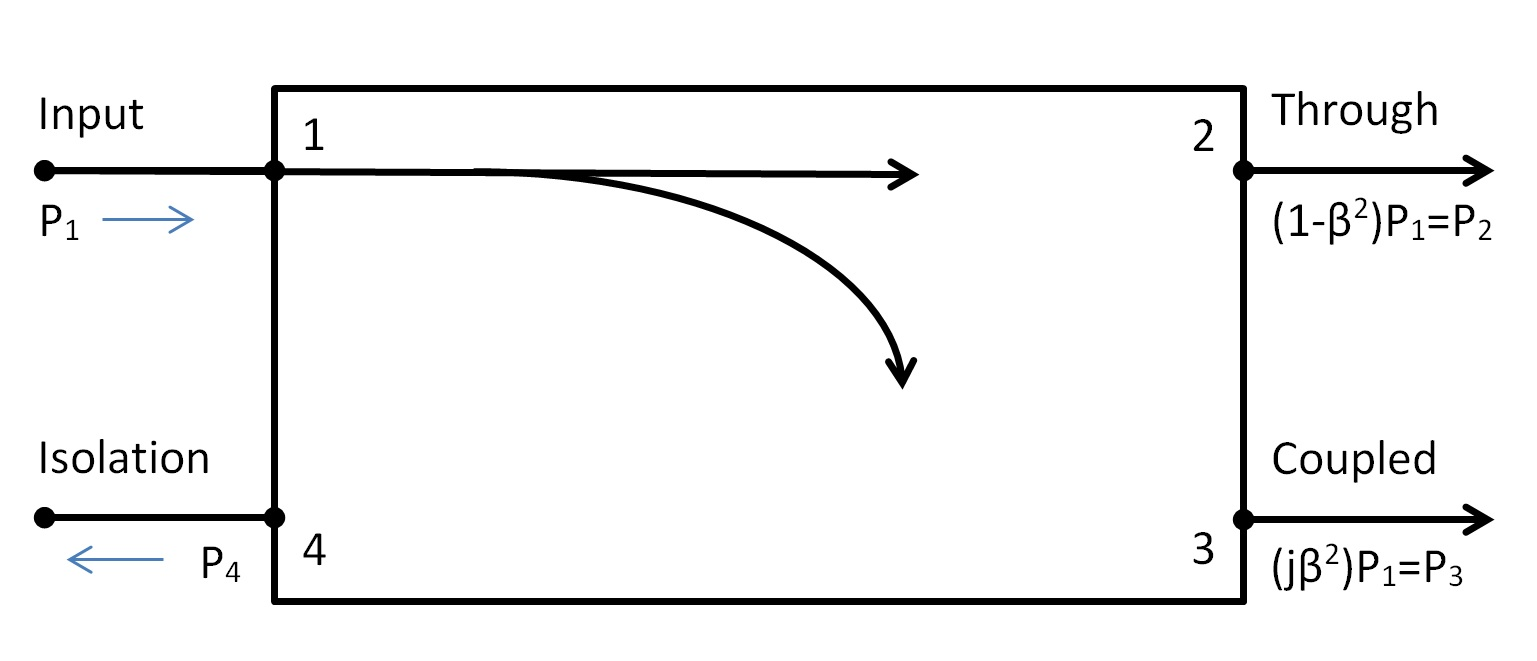
\includegraphics[width=.8\textwidth,keepaspectratio]{images/directionalcoupler.png}\caption{Směrová odbočnice, převzato z \cite{widebandcouplers}.}\label{directionalcoupler}\end{figure}	

	Pomocí tradičních odbočnic jako na obr. \ref{directionalcoupler} je možné provádět separaci s velkou izolací nechtěného signálu, ovšem nesplňují požadavek na šířku zpracovávaného pásma \cite{widebandcouplers}. Problematická je také skutečnost, že s rostoucí šířkou použitelného pásma odbočnice obvykle klesá směrovost odbočnice. Dochází tedy pouze k částečné separaci, další separační krok by byl nezbytný během zpracování naměřených dat.
	
	\item
	\textbf{Odporový můstek}\\*	
	\begin{figure}[htbp]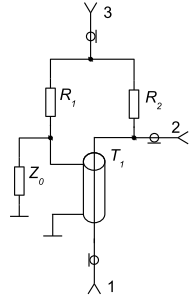
\includegraphics[width=\textwidth,height=5cm,keepaspectratio]{images/resistivebridge.png}\caption{Odporový směrový můstek, převzato z \cite{resistivedirectionalbridge}.}\label{resistivebridge}\end{figure}	
	Pomocí odporových můstků je možné provádět separaci signálů s velmi velkou šířkou pásma, např. v \cite{resistivedirectionalbridge} a obr. \ref{resistivebridge} uveden můstek pro pásmo \SI{300}{\kilo\hertz}--\SI{13.5}{\giga\hertz}. Opět ovšem nejsou signály plně separovány, je nezbytný další separační krok během zpracování.
	
	\item
	\textbf{Časové oddělení}\\*	
	Pokud má budicí signál tu vlastnost, že má omezenou délku, po kterou se mění a mimo ni je konstantní (vybraný jednotkový skok tuto vlastnost splňuje), je možné jej od odrazů separovat tak, že je časově posunut vůči odezvě systému. Toho je možné dosáhnout například použitím dokonalého vedení bez odrazů, které se zapojí mezi bod měření a měřený systém. Jeho délka musí být minimálně taková, aby se nemohla nikdy překrývat nekonstantní část budicího signálu s odrazy. Pokud je v naměřených datech známá poloha budicího pulzu (nebo je-li možné jej spolehlivě identifikovat), je možné naměřená data rozdělit na část buzení a část odpovědi měřeného systému. První část pak může sloužit ke korekci frekvenční charakteristiky změřené odezvy systému a odhadu šumového spektra. Známe-li i přesnou délku prodlužovacího vedení (hrubě z návrhu zařízení, přesně pomocí kalibrace), je možné provést kalibraci měřicí roviny. Při použití této metody separace stačí vzorkování pouze jednoho průběhu, snižuje tedy počet potřebných vzorkovačů ze dvou (nebo více) na jeden. Z toho také vyplývá, že měřená data nejsou zatížena chybou, která by mohla vzniknout vzhledem k rozdílným vlastnostem jednotlivých vzorkovačů.
	
	Na obrázku \ref{separableunitstep} je znázorněna odezva na chybovou funkci. Buzení se nachází v čase $t=0$, odezva v čase $t=0.5$. Průběh budicí funkce je předem známý, nekonstantní část průběhu se nepřekrývá s odezvou, je tedy možné je v časové oblasti $t\in (0;0.5)$ rozdělit na dva samostatné průběhy.

\begin{figure}[htbp]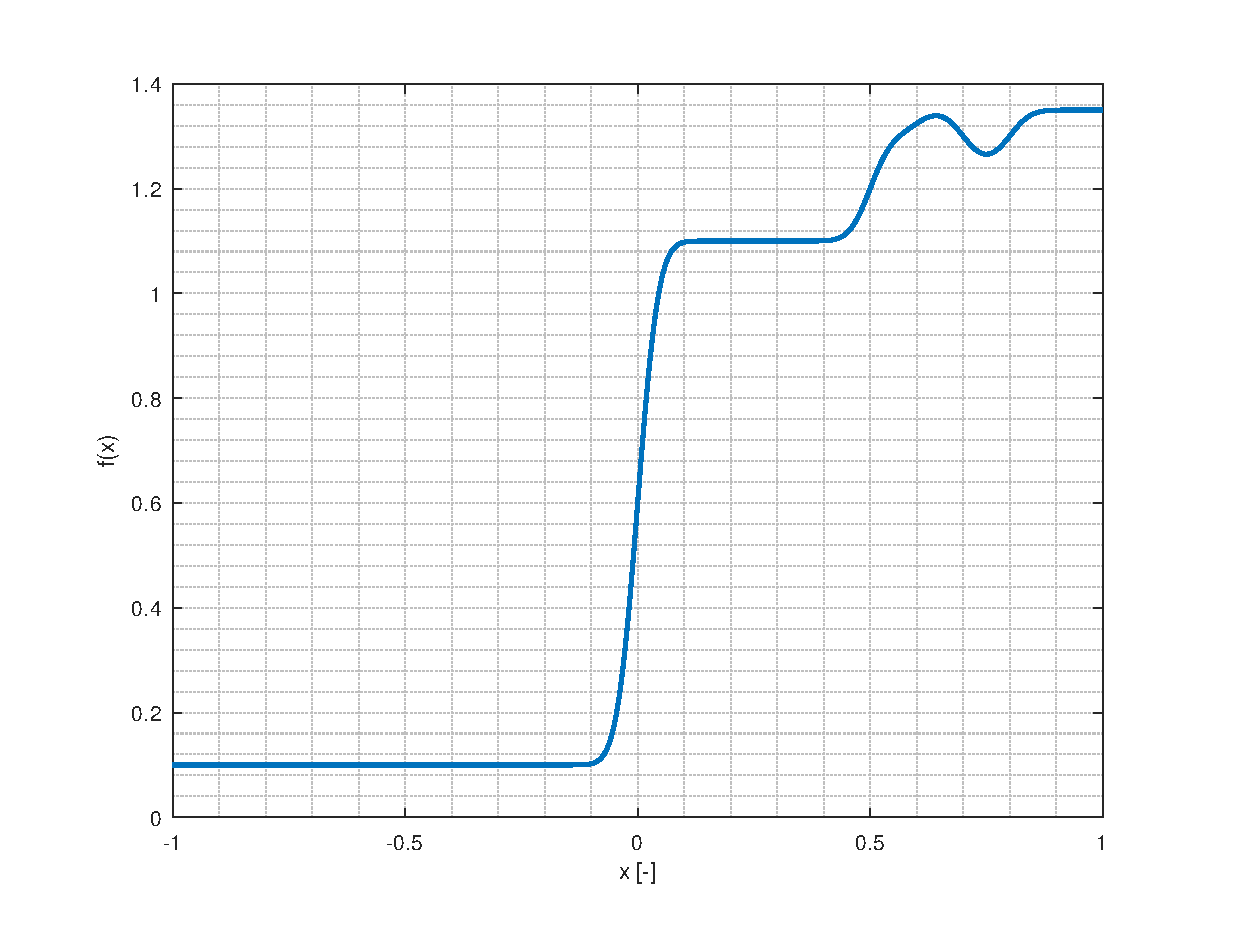
\includegraphics[width=\textwidth,keepaspectratio]{images/separableunitstep.eps}\caption{Časově oddělitelná odezva na jednotkový skok.}\label{separableunitstep}\end{figure}	
\end{itemize}

Pro vybraný budicí signál (jednotkový skok) je tedy možné provést separaci od odrazů zpožďovacím vedením a vhodným rozdělením naměřených dat na dvě části. Toto řešení se jeví jako obvodově i výpočetně nejjednodušší z uvažovaných metod separace.
\chapter{Rozšíření dynamického rozsahu, potlačování šumu a rušení}
Pro co nejpřesnější měření je nezbytné dosáhnout co největšího SNR (signal to noise ratio). Prvním limitujícím faktorem je dynamický rozsah ADC. V případě měření v reálném čase by bylo možné použít nanejvýš osmibitové převodníky, které mají dynamiku přibližně \SI{48}{\deci\bel} podle vztahu \ref{equation_dynamic_range}.
\begin{equation}
	 DR_n=20\log\left(2^n-1\right)
	 \label{equation_dynamic_range}
\end{equation}
Pro nižší rychlosti jsou dostupné již ADC s vyšší přesností, někdy již integrované přímo do mikrokontrolérů. Běžně se integrují převodníky až do \SI{1}{\megasample} při rozlišení 12~bitů, tedy s dynamickým rozsahem přibližně
\begin{equation}
	DR_{12}\doteq \SI{72}{\deci\bel}
\end{equation}

Pro aplikace ve zvukové technice jsou pak dostupné šestnáctibitové až dvacetičtyřbitové převodníky (obvykle do \SI{96}{\kilosample}) s dynamikou od 
\begin{equation}
	DR_{16}\doteq \SI{96}{\deci\bel}
\end{equation} až do
\begin{equation}
	DR_{24}\doteq \SI{144}{\deci\bel}
\end{equation}
 Druhý údaj je však pouze teoretický, převodníky sice nabízejí tento počet bitů, ovšem jejich vlastní šum zpravidla omezuje použitelný rozsah na méně než \SI{100}{\deci\bel}. Přesné \SI{24}{\bit} převodníky, které mají skutečně dynamický rozsah odpovídající počtu bitů, vzorkují zpravidla nanejvýš na desítkách \si{\hertz}. Takové rychlosti jsou však pro použití v reflektometru příliš pomalé, neboť změření odezvy systému by bylo velice zdlouhavé.

Vzhledem k rychlosti se zdají být použitelné nanejvýš \SIrange{12}{16}{bitové} převodníky. Existují ovšem metody rozšíření dynamického rozsahu, zpravidla spoléhající na zkreslení měřených dat nelineární funkcí, která umožní navzorkovaná data inverzní funkcí převést zpět na původní signál, přičemž ale nedojde ke ztrátě přesnosti, nýbrž k jejímu zlepšení v určité části převodní charakteristiky. Pro účely telefonie se v minulosti používaly například komprese definované ve standardu G.711 od ITU-T. Tyto komprese umožňovaly komprimovat logaritmicky enkódovaná data z 14~bitů na 8, přičemž uživatel po dekompresi pozoroval výrazně menší zkreslení, než k jakému by došlo, pokud by bylo použita přímo osmibitová kvantizace.

Pro účely měření vysokofrekvenčních signálů se vyrábí logaritmické detektory s rozsahem až \SI{100}{\deci\bel} \cite{AD8309datasheet} \ref{ad8309function}. Pro nízké frekvence poskytuje např. detektor AD8309 \SI{85}{\deci\bel} dynamického rozsahu při toleranci $\pm \SI{1}{\deci\bel}$, tolerance je zakreslena v grafu \ref{ad8309error}. Logaritmus je prostá funkce, je tedy možné spočítat její inverzní funkci. Podle \ref{ad8309function} odpovídá vstupnímu rozsahu \SIrange{-70}{10}{\deci\bel m} výstupní rozsah o velikosti \SI{1.5}{\volt}. Při uvažování převodníku s referencí \SI{3.3}{\volt} a rozlišení 12~bitů odpovídá nejmenší měřitelný rozdíl napětí převodníkem \SI{0.8}{\milli\volt}, což s detektorem odpovídá vstupnímu rozlišení přibližně \SI{0.043}{\deci\bel}. Kombinací takového detektoru s dvanáctibitovým převodníkem a proložením dat získaných z lineárního a logaritmického měření je možné vytvořit převodník, který se přesností blíží rychlému šestnáctibitovému převodníku.

\begin{figure}[htbp]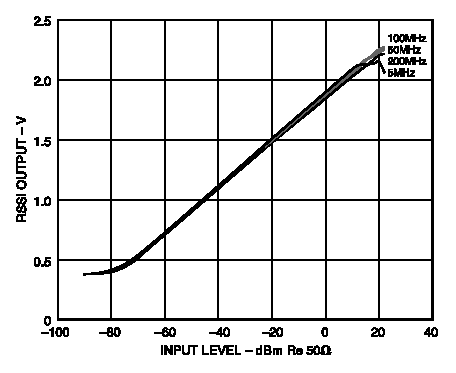
\includegraphics[width=0.8\textwidth,keepaspectratio]{images/AD8309_function.eps}\caption{Převodní funkce logaritmického detektoru AD8309 \cite{AD8309datasheet}}\label{ad8309function}\end{figure}	

\begin{figure}[htbp]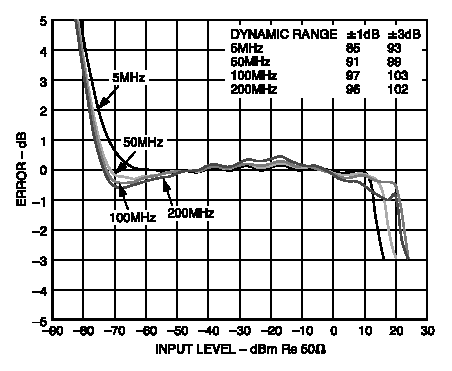
\includegraphics[width=0.8\textwidth,keepaspectratio]{images/AD8309_error.eps}\caption{Chyba převodní funkce logaritmického detektoru AD8309 \cite{AD8309datasheet}}\label{ad8309error}\end{figure}

Pro potlačení šumu v měřeném průběhu je možné použít velké převzorkování signálu a aplikovat na tato data filtr pro potlačení šumu mimo užitečné pásmo. Dále je možné měřený průběh opakovaně měřit a statisticky zpracovávat (buď jednoduchým průměrem nebo např. Kalmanovými filtry).

Použitím měření v ekvivalentním čase je také možné redukovat rušení z okolí za předpokladu, že žádný násobek tohoto rušivého signálu není přesně roven vzorkovacímu kmitočtu. Pak se toto rušení projeví jako šum, který je možné odstranit či alespoň potlačit metodami zmíněnými v předchozím odstavci. V opačném případě je možné rušení potlačit pouze tak, že se provede měření s jinou vzorkovací frekvencí.
\chapter{Navržené blokové zapojení reflektometru}
V předchozích kapitolách byly vysvětleny technologie, které byly uvažovány pro návrh architektury jednoduchého reflektometru a následně byly z nich vybrány ty nejvhodnější nebo nejjednodušší na implementaci. Pro jednotlivé části reflektometru tedy budou použity tyto stavební bloky:
\begin{itemize}
	\item
	\textbf{Buzení}\\*
	Pro buzení bude použito buzení aproximovaným jednotkovým skokem pomocí budiče technologie \acrshort{CML}, kterým je možné dosáhnout aproximace s náběžnou hranou o délce kratší než \SI{100}{\pico\second}, typicky okolo \SI{60}{\pico\second}, tedy s užitečnou šířkou pásma v jednotkách \si{\giga\hertz}. Výstup je dobře přizpůsoben pro použití v \SI{50}{\ohm} systémech.
	
	\item
	\textbf{Separace budicího a odraženého signálu}\\*	
	Pro separaci buzení od odezvy systému bude použito prodlužovací vedení jako metoda pro dosažení časového posunu. Samotná separace bude probíhat až z navzorkovaných dat během zpracování.
	
	\item
	\textbf{Vzorkování}\\*	
	Data budou sbírána pomocí postupného vzorkování v ekvivalentním čase pomocí vyvážených diodových můstků. Touto metodou je možné vzorkovat měřený signál pomocí pomalých převodníků s větším dynamickým rozsahem a přesností, je také možné potlačit ruchy z okolí. Byla navržena metoda pro měření s dynamickým rozsahem nejméně \SI{80}{\deci\bel}.
	
	\item
	\textbf{Generování signálů pro řízení reflektometru}\\*	
	Pro řízení jednotlivých částí reflektometru bude použita \acrshort{PLL} Si5351, která disponuje 8 výstupy, které je možné konfigurovat jako diferenciální výstupy. Jednotlivé výstupy mohou mít neceločíselné vzájemné poměry frekvencí (krok nastavení je menší než \SI{1}{ppm}), je možné dosáhnout vzorkování s krokem menším než \SI{100}{\pico\second}, tedy ekvivalentní vzorkovací frekvence větší než \SI{10}{\gigasample}. Díky proudovým výstupům je možné ji přímo propojit jak se vstupy \acrshort{CML} logických prvků, tak ji použít pro spínání diodových vzorkovačů. Je možné i vygenerovat synchronizační hodinový signál pro mikrokontrolér, aby se provádělo vzorkování v přesně stanovený čas.
\end{itemize}

Z těchto jednotlivých prvků je tedy již možné navrhnout základní blokové zapojení navrhované architektury.

\begin{figure}[htbp]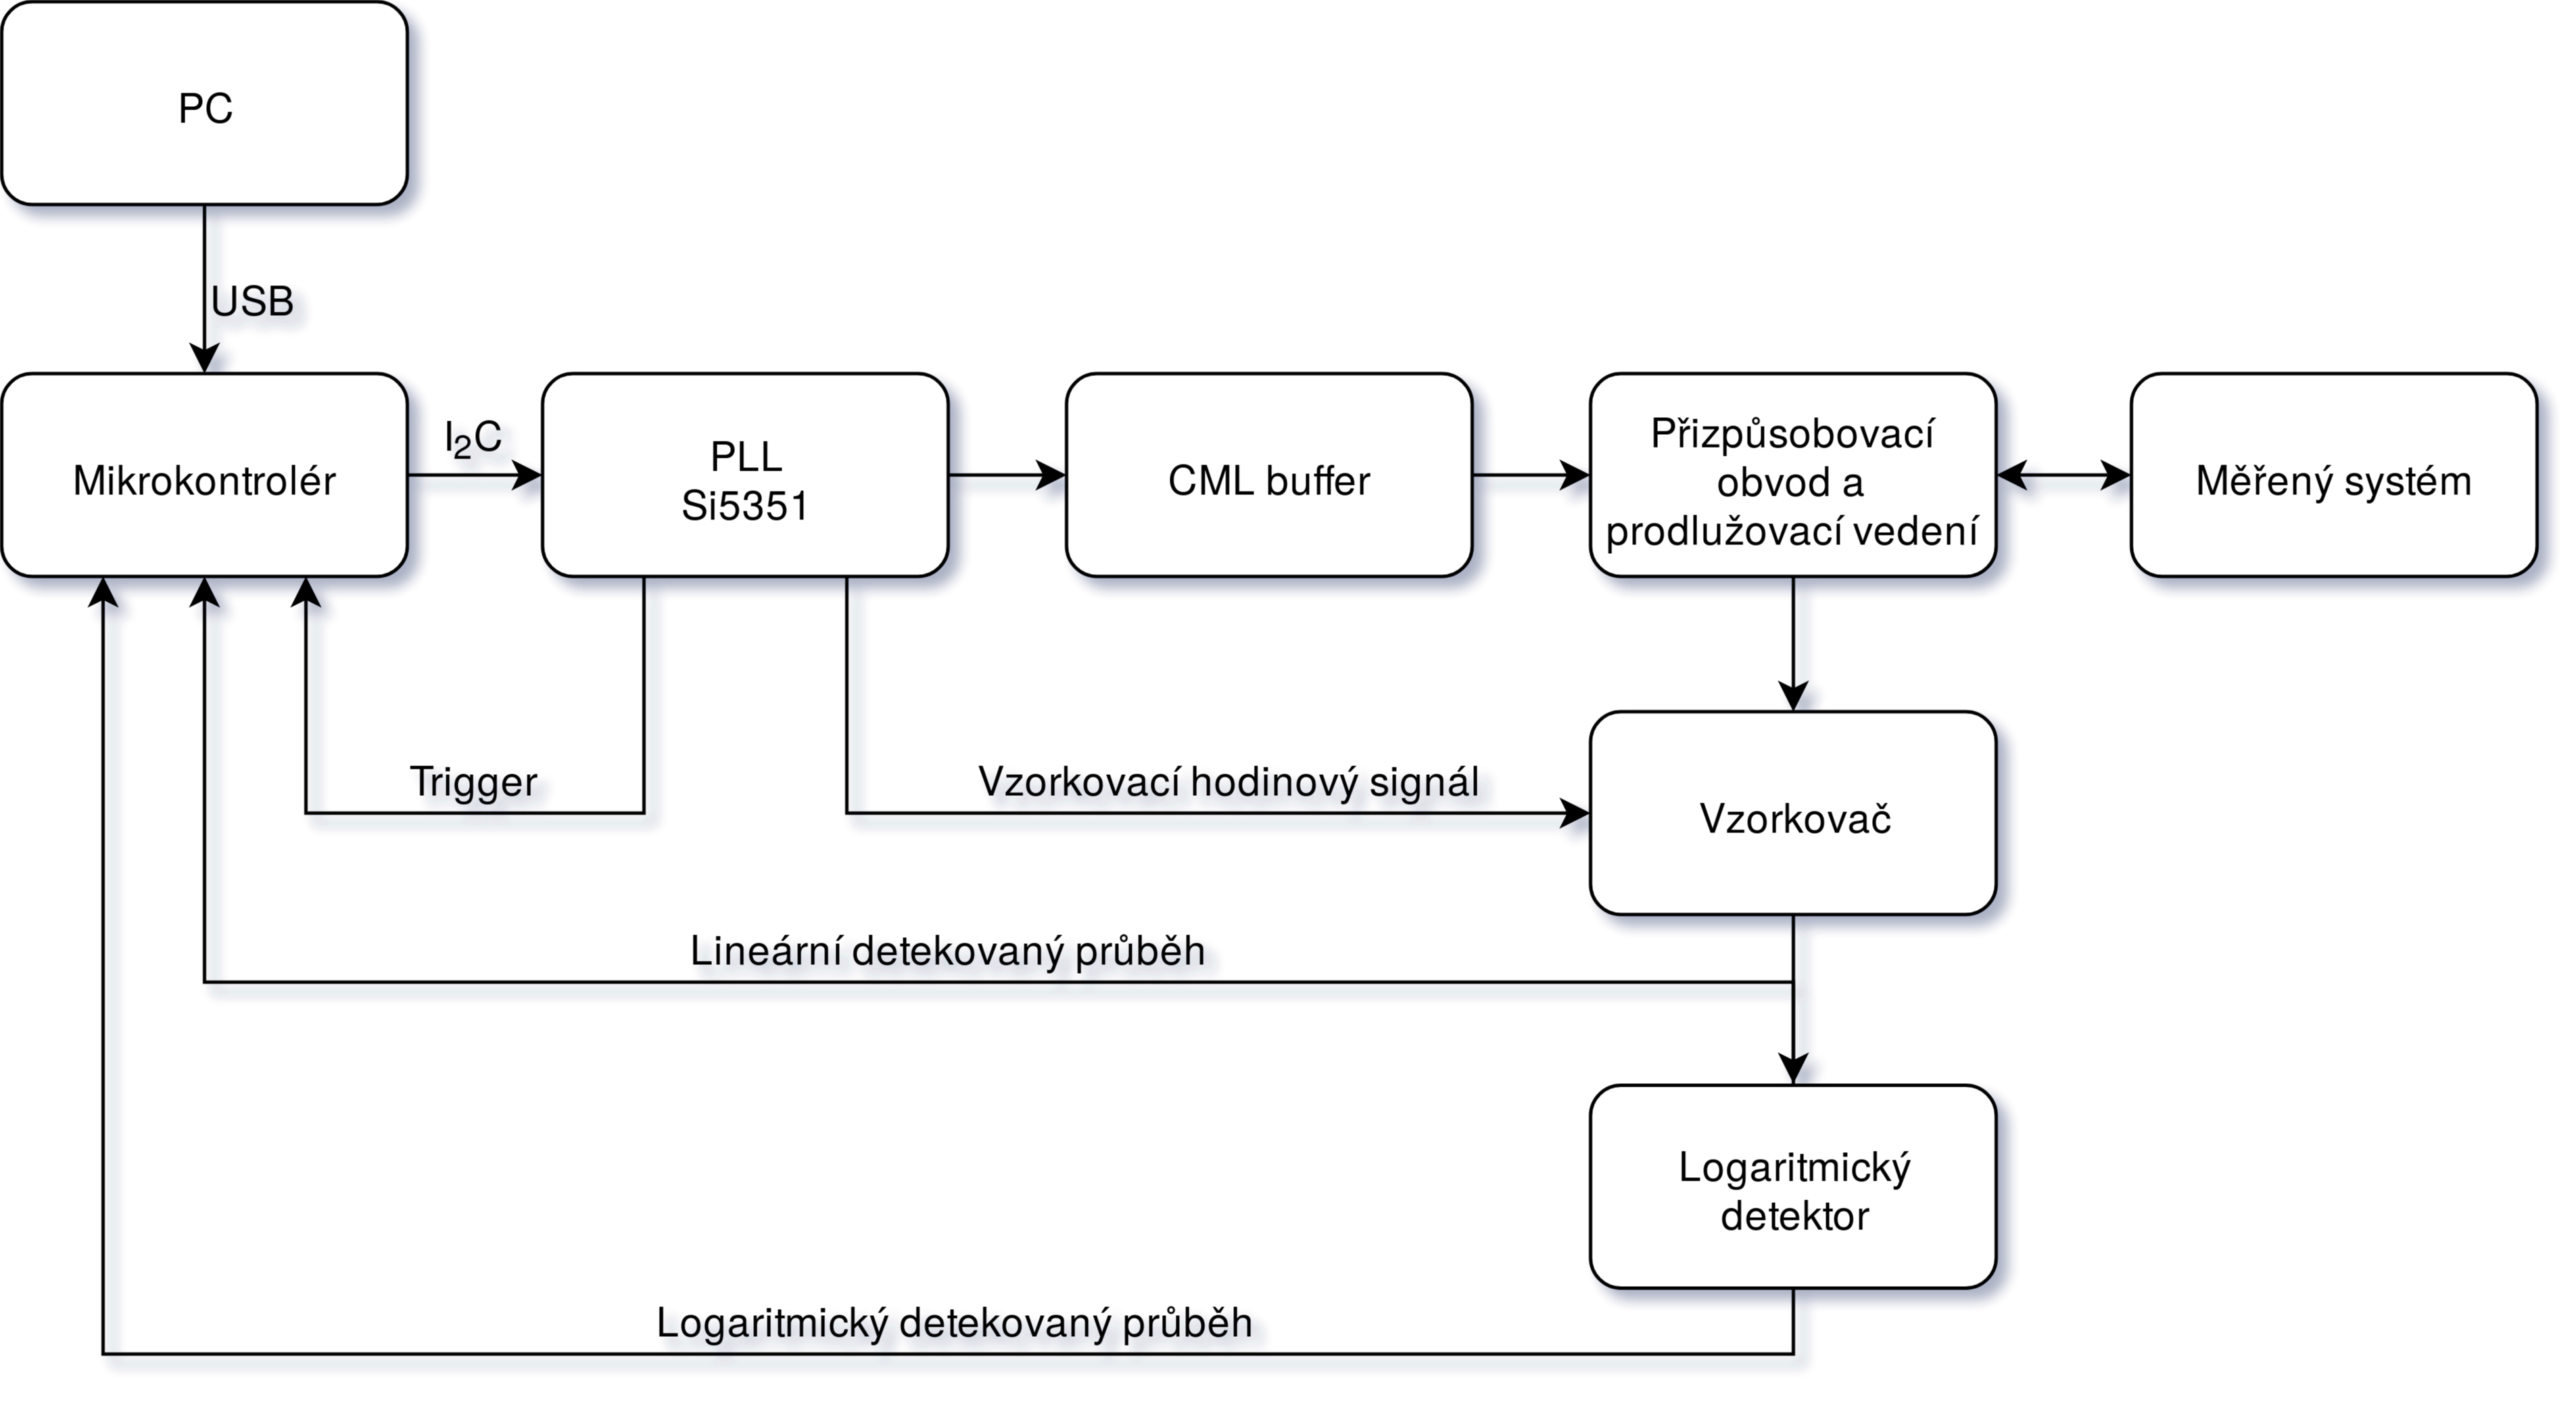
\includegraphics[width=\textwidth,keepaspectratio]{images/reflectometer_blockdiagram_simple.png}\caption{Základní blokové schéma navržené architektury reflektometru.}\label{reflectometer_blockdiagram}\end{figure}
\input{diplomovy_projekt_7_zaver.tex}

\appendix

\printindex

\bibliographystyle{amsalpha}
\bibliography{diplomovy_projekt}

%\ctutemplate{specification.as.chapter}

\end{document}